\documentclass[a4paper,10pt]{article}
\usepackage[T2A]{fontenc}
\usepackage{sectsty}
\usepackage{changepage}
\usepackage{filecontents}
\usepackage{array}
\usepackage{float} 
\usepackage{subcaption}
\usepackage[utf8]{inputenc}
\usepackage{physics} 
\usepackage{graphicx}
\usepackage{enumerate}
\graphicspath{{../misc/}}
\usepackage{setspace,amsmath}
\usepackage{bigstrut}
\usepackage{tabularx}
\usepackage[left=15mm, right=15mm, top=15mm, bottom=15mm]{geometry} 
\usepackage[nottoc]{tocbibind}
\usepackage[
style=chem-biochem,
sorting=nyt,
backend=biber,
defernumbers=false,
citestyle=authoryear
]{biblatex}

\usepackage{multicol}
\DeclareBibliographyAlias{misc}{article}
\addbibresource{lit.bib} 
%%%%%%%%%%%%%%%%%%%%%%%%%%%%%%%%%%%%%

\makeatletter
\def\@makefnmark{\hbox{\@textsuperscript{\normalfont(\@thefnmark)}}}
\makeatother
 
\captionsetup[figure]{labelsep=period, labelfont=bf, labelformat=simple}
\captionsetup[subfigure]{labelsep=period, labelfont=bf, labelformat=simple} 
\captionsetup[table]{labelsep=period, labelfont=bf, labelformat=simple}
% \renewcommand*{\thesubfigure}{\alph{subfigure}}
\renewcommand{\ref}{\textbf{\ref{}}}
\usepackage{titling,lipsum}

\usepackage{amsmath}
\usepackage{bm}

\usepackage{hyperref}
\hypersetup{
    colorlinks,
    citecolor=black,
    filecolor=black,
    linkcolor=black,
    urlcolor=blue
}

\begin{document}

\thispagestyle{empty}

\begin{center}
    \huge\textbf{Training inhibitory connections between local receptive fields in spiking neural networks}\\
\end{center}

\begin{center}
\begin{tabular}{ccc}
\large{D. Gafni \textsuperscript{a\textasteriskcentered}} & \large{D.V. Nekhaev \textsuperscript{b}} & \large{V.A. Demin \textsuperscript{b}} \\
\end{tabular}

\textsuperscript{(a)} Lomonosov Moscow State University, Moscow, Russia \linebreak
\textsuperscript{(b)} National Research Center <<Kurchatov Institute>>, Moscow, Russia \linebreak
\textsuperscript{(\textasteriskcentered)} Corresponding author. Email adress: \textit{danielgafni16@gmail.com}


\end{center}

\section*{Acknowledgments}
This work was partially supported by the Russian Science Foundation (project № 20-79-10185) in the studying of inhibitory connections training and by the Russian Foundation for Basic Research (Grant No. 18-29-23041) in the part of comparison of convolгtional and locally connected achitectures.

\addcontentsline{toc}{section}{Abstract}
\section*{Abstract}
Standard learning methods (based on the error backpropagation) used in artificial neural networks (ANNs) are difficult to apply to spiking neural networks (SNNs) due to discrete and time-distributed nature of the events they generate. Although such projects exist, local learning algorithms, which are more biologically correct, capable of performing unsupervised learning and more energy efficient (if implemented on specialized hardware), are of greater interest.

SNN's local learning rules are significantly understudied in comparison to ANNs, and because of this, SNN-based alrorithms produce lower inference quality metrics. Thus, the study of SNN learning algorithms, like spike-timing-dependent-plasticity (STDP), for use in various SNN architectures is an important problem.

The introduction of inhibitory connections (with negative weights) allows to achieve a better distinction of features learned by the neurons. In this work it is shown that learning competition relationships in a locally connected (LC) SNN potentially leads to higher pattern recognition accuracy due to the organization of competition and cooperation between groups of neurons. It is also shown that the LC SNN produces better results than a convolutional SNN.

\section*{Keywords}
Spiking Neural Networks, Unsupervised Learning, Inhibitory Connections, Neuroscience

\section*{Declarations}

\begin{flushleft}
 \begin{tabularx}{\textwidth}{lm{10cm}}
  \textbf{Funding} & {This work was partially supported by the Russian Science Foundation (project № 20-79-10185) in the studying of inhibitory connections training and by the Russian Foundation for Basic Research (Grant No. 18-29-23041) in the part of comparison of convolгtional and locally connected achitectures.} \\
  \textbf{Data, Materials, Code} & {\href{https://github.com/danielgafni/bachelor}{https://github.com/danielgafni/bachelor}} \\
  \textbf{Conflicts of Interest} & {The authors declare no conflict of interest.} \\
 \end{tabularx}
\end{flushleft}

\pagebreak 

\addcontentsline{toc}{section}{Introduction}
\section*{Introduction}

Modern abstract neural networks (represented by combinations of linear layer transformations and non-linear activation functions) do an excellent job at solving many machine learning problems \parencite{pmlr-v28-wan13, Khan_2020}. However, training them is a laborious process that requires large computational resources. Typically, training is conducted using hundreds or thousands of examples and can take months. Both training and inference of formal neural network algorithms are far from being effective \parencite{Edwards2015GrowingPF}. This is due both to the physically separate storage of connection weights and neuron activations, and to the calculations themselves, which are tensor in nature, associated with vector-matrix and matrix-matrix multiplication of floating point numbers. Modern CPUs are not optimized for this kind of computing. GPUs --- architectures originally created for working with computer graphics, and therefore more suitable for tensor calculations --- are much better at these tasks than traditional CPUs, but they do not perform with the desired efficiency either. The number of parameters in modern formal neural networks can reach tens \parencite{ManyParams, Khan_2020} and even hundreds of billions (the latest OpenAI language model GPT-3 \parencite{brown2020language}).

Spiking neural networks (SNNs) are an alternative promising neuromorphic algorithm and have several advantages over formal neural networks.

\begin{itemize}
\item SNNs allow a richer dynamic coding of patterns in continuous time, which is usually not available for formal neural networks \parencite{Ismail_Fawaz_2019}. Thus, SNNs are of greatest interest for solving time series problems (video and sound streams processing, speech recognition, decision making).

\item Local algorithms, which use only information from the neurons connected by this connection to update the weight of each connection \parencite{STDP, pehlevan2019spiking, Baldi_2016}, can be used to train SNNs. On the contrary, when training formal neural networks, information about all neural connections between this connection and the output of the network is used to update the weight of each connection. Thus, SNNs learning algorithms on their own are far more efficient than formal neural network learning algorithms.

\item Moreover, these algorithms can use unsupervised learning, which does not require manual data labeling, as in the case of backpropagation methods.

\item SNNs can be implemented on specialized neuromorphic processing units (both based on digital elements \parencite{TrueNorth, Loihi, Akida} and using hybrid digital-analog circuits (BrainScales, \parencite{SpiNNaker}), including those based on memristors \parencite{WANG2020101809}, which have ultra-low power consumption (achieved by reducing the number of acts and the average length of signal transmission, as well as the spatial and temporal sparseness of spikes in the network). This implementation, together with the algorithmic advantage of the SNNs, also provides significant performance gains. \parencite{hardware1, hardware2}.

\item SNNs, to a greater extent than formal neural networks, biologically correctly model the interactions of neurons, which can be used for biological simulations of the nervous system for the purposes of studying not only bioinformatics, but also biophysical and medical aspects of its functioning.
\end{itemize}

It is of interest to study well-known ANN architectures in application to SNN, such as convolutional, locally connected and fully connected \parencite{Khan_2020} architectures. Moreover, the introduction of additional recurrent inhibitory connections contributes to a better separation of features in the learning process \parencite{MaxActiv1, MaxActiv2}. A fully connected network is the simplest model that can be used as a benchmark. Convolutional and locally connected architectures use convolution --- an operation that allows to extract important features more efficiently (comparing to a fully connected network). The locally connected architecture is especially interesting, because it can be easily implemented in hardware, since, unlike a convolutional network, it does not use shared synaptic weights  inside a separate feature map. A locally connected architecture has significantly fewer parameters than a fully connected architecture and allows to train a unique set of features for each receptive field, in contrast to convolutional networks. At the same time, convolutional networks have translational invariance, a useful property for image processing (spatially correlated data). The presence of competition in the SNN makes it possible to make their features more independent. Therefore, for experiments in this work, we chose locally connected SNNs with inhibitory connections, and as basic models, convolutional and fully connected networks with inhibitory connections. We:

\begin{enumerate}[i]

\item compare this architecture with a Convolution Spiking Neural Network (CSNN) and a Fully Connected Spiking Neural Network (FCSNN).

\item study the effect of training the inhibitory connections \parencite{MaxActiv1, MaxActiv2, hardware_survey} between neurons on the accuracy of the image classification problem of handwritten digits from the MNIST \parencite{MNIST} dataset for the architecture of a locally connected network (Locally Connected Spiking Neural Network, LCSNN) \parencite{saunders2019locally};

\end{enumerate}

\clearpage

\section{Training of the SNN with fixed inhibitory connections of local receptive fields}

\subsection{Problem description}
For different networks architectures comparative analysis, a classical machine learning problem was chosen --- the problem of classifying images of handwritten digits from the MNIST dataset. MNIST consists of labeled training and test subsets of 60,000 and 10,000 images. The images have 28 $ \times $ 28 resolution and are black and white. Due to the need to calibrate the networks (see below), the original training subset was split into 50,000 images for training (training dataset) and 10,000 images for calibration (calibration dataset).

The images are also cropped so that only the center 20 $ \times $ 20 pixels are used. \\

\subsection{Competition between local receptive fields in SNN}
In this paper, networks are studied using locally connected, fully connected and convolutional layers. In a fully connected layer, each neuron is connected to each neuron from the previous layer. In the convolutional layer, neurons are divided into channels. The neurons in one channel have shared weights, but each neuron is only connected to a certain region (rectangular in the case of a two-dimensional layer) \parencite{li2020survey} --- receptive field, or patch. The architecture of the locally connected layer is the same, but each neuron has its own unique weights \parencite{saunders2019locally}.

The neural network architecture of LCSNN is inspired by the structure of the visual cortex of the brain. The $Y$ network layer consists of $n$ channels, each of which is locally connected to the $X$ layer of neurons, and neurons with common receptive fields are connected by inhibitory connections (Fig. \ref{fig:LC_SNN_architecture}).

\begin{figure} \label{LCSNN}
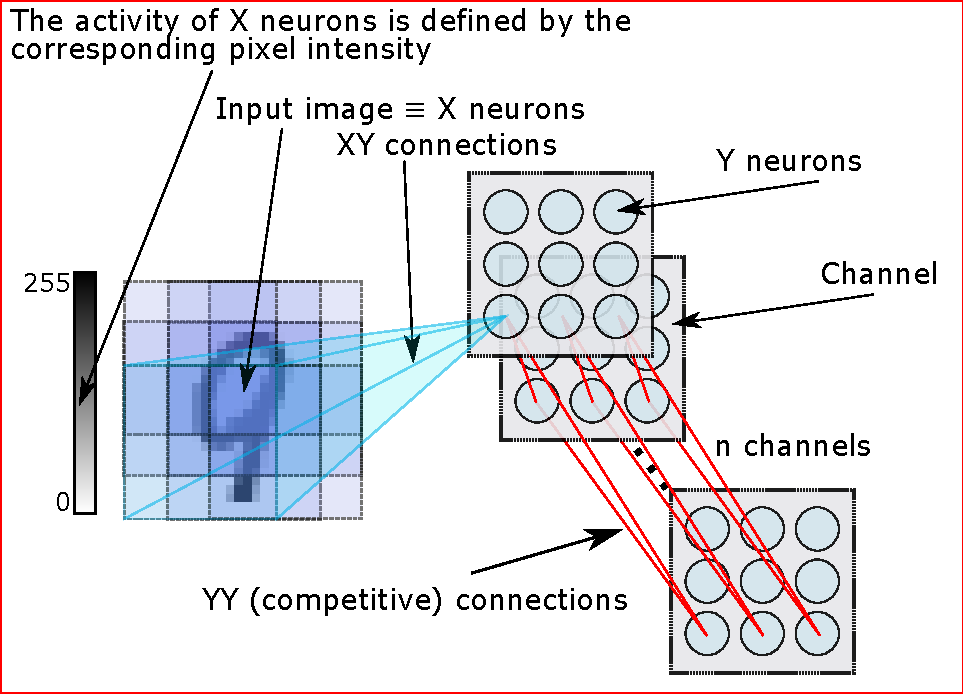
\includegraphics[,
 width=\textwidth,keepaspectratio=true]{LCSNN.pdf} 
    \caption{LCSNN architecture}
    \label{fig:LC_SNN_architecture}
\end{figure}

Such connections have negative weights, which means they negatively affect neuron activity. Neurons that do not have a common patch (and therefore respond to different areas of the image) do not compete with each other. Inhibitory connections are introduced to improve the separation of neurons by learned features. A similar architecture can be built for networks with convolution or fully connected layers. We studied networks with the number of $Y$ neurons $\approx$ 100 --- 900 and folowwing convolutions parameters: kernel size of 8 or 12 and stride of 4. Since the MNIST images were cropped to a size of 20 $\times 20$, the number of neurons per the channel was 3 or 4.

This work uses the Adaptive Integrate-And-Fire (ALIF) model of neurons. The dynamics of the neuron potential in this model is given by the equation

\begin{equation} \label{eq:alif}
 \tau_v \dv{v(t)}{t} = -v(t) + v_{rest} + I(t) \cdot R \text{,}
\end{equation} where $I(t)$ is the current, accumulated by time moment $t$, $v_{rest}$ --- relaxation level, $\tau_v$ --- simulation time constant, а $R$ --- unit coefficient, numerically equal to one.\\ 

Activation threshold $v_{thresh}$ of an ALIF neurone is not static, but slightly increases with every spike, then relaxing to its initial value $\theta_o$. The dynamics of the activation threshold is given by:
\begin{equation} 
 v_{thresh} = \theta_0 + \theta(t) \text{,}
\end{equation} where $\theta_0$ is the initial activation threshold, $\theta(t)$ --- an adaptive additive to the activation threshold after each spike generation, which is calculated from the condition\\

\begin{equation}
 \tau_v \dv{\theta(t)}{t} = -\theta(t)
\end{equation}\\

After the generation of each spike, a short refractory period occurs, when for time $t_{refract}$ the potential of the neuron remains at the level of $v_{reset}$. The initial connection weights are generated randomly from a uniform distribution.

\subsection{Forward connections training}
To reduce the number of model parameters, images are cropped to 20 $\times$ 20 pixels. The edges of the images are often almost empty, so this operation has little or no effect on the amount of information, available to the network. For each image, $X$ spikes are generated using a Poisson distribution with a mathematical expectation value  proportional to the corresponding pixel intensiveness. Connections $XY$ are trained according to the STDP \parencite{STDP} rule. This is a biologically inspired rule of unsupervised learning. When the presynaptic spike (pre-spike) is received and the post-spike is emitted, the weight $w$ of the corresponding connection is increased by $ \Delta w $, where
\begin{equation} 
\Delta w =
 \begin{cases}
 A_+ \cdot e^{- \frac{t_{pre} - t_{post}}{\tau_+}}, t_{pre} - t_{post} > 0\\
 A_- \cdot e^{- \frac{t_{pre} - t_{post}}{\tau_-}}, t_{pre} - t_{post} < 0
 \end{cases}
\end{equation}

Let's notice, that

$$
\begin{cases}
 A_{+} > 0\\
 A_{-} < 0
\end{cases}
$$

Thus, in the process of learning, the weights of connections where pre-spikes are systematicly recieved right before the emmision of post-spikes are increased, and decreased if vice versa. After such training, the neurons begins to actively react to pre-spikes received from neurons with larger connection weights. This leads to the neuron weights learning certain features (Fig. \ref{fig:training}). If these pre-spikes are recieved in a short enough time period, they might cause a new spike. The opposite rule (with $A_{+}$ and $A_{-}$ having the opposite signs) is called the anti-STDP \parencite{anti-STDP} rule. It is used to train inhibitory connenctions in section \ref{section:competition-training} of this paper.

After each training iteration, the weights are normalized to keep their sum equal to a certain constant. This is done to forbid the weights to grow too large. The value of the normalization constant is an important model hyperparameter that has to be carefully selected for each specific network architecture.

\begin{figure}
\centering
\begin{subfigure}{0.45\textwidth}
    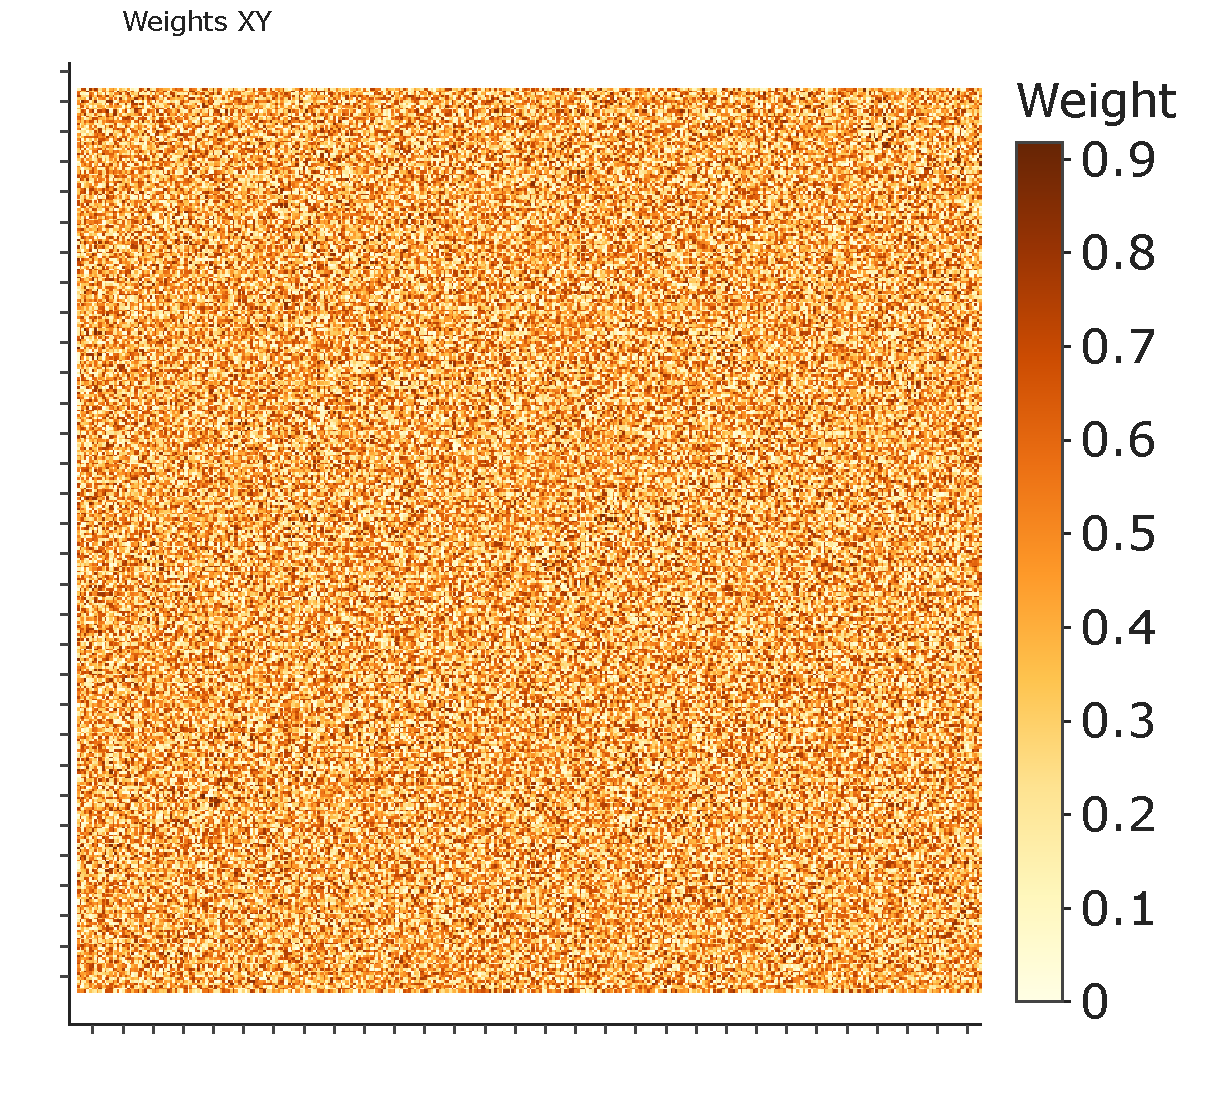
\includegraphics[width=\textwidth,keepaspectratio=true]{weights_XY_untrained.pdf} 
    \caption{}
    \label{fig:training:before_training}
\end{subfigure}
\begin{subfigure}{0.45\textwidth}  \label{weights_XY}
    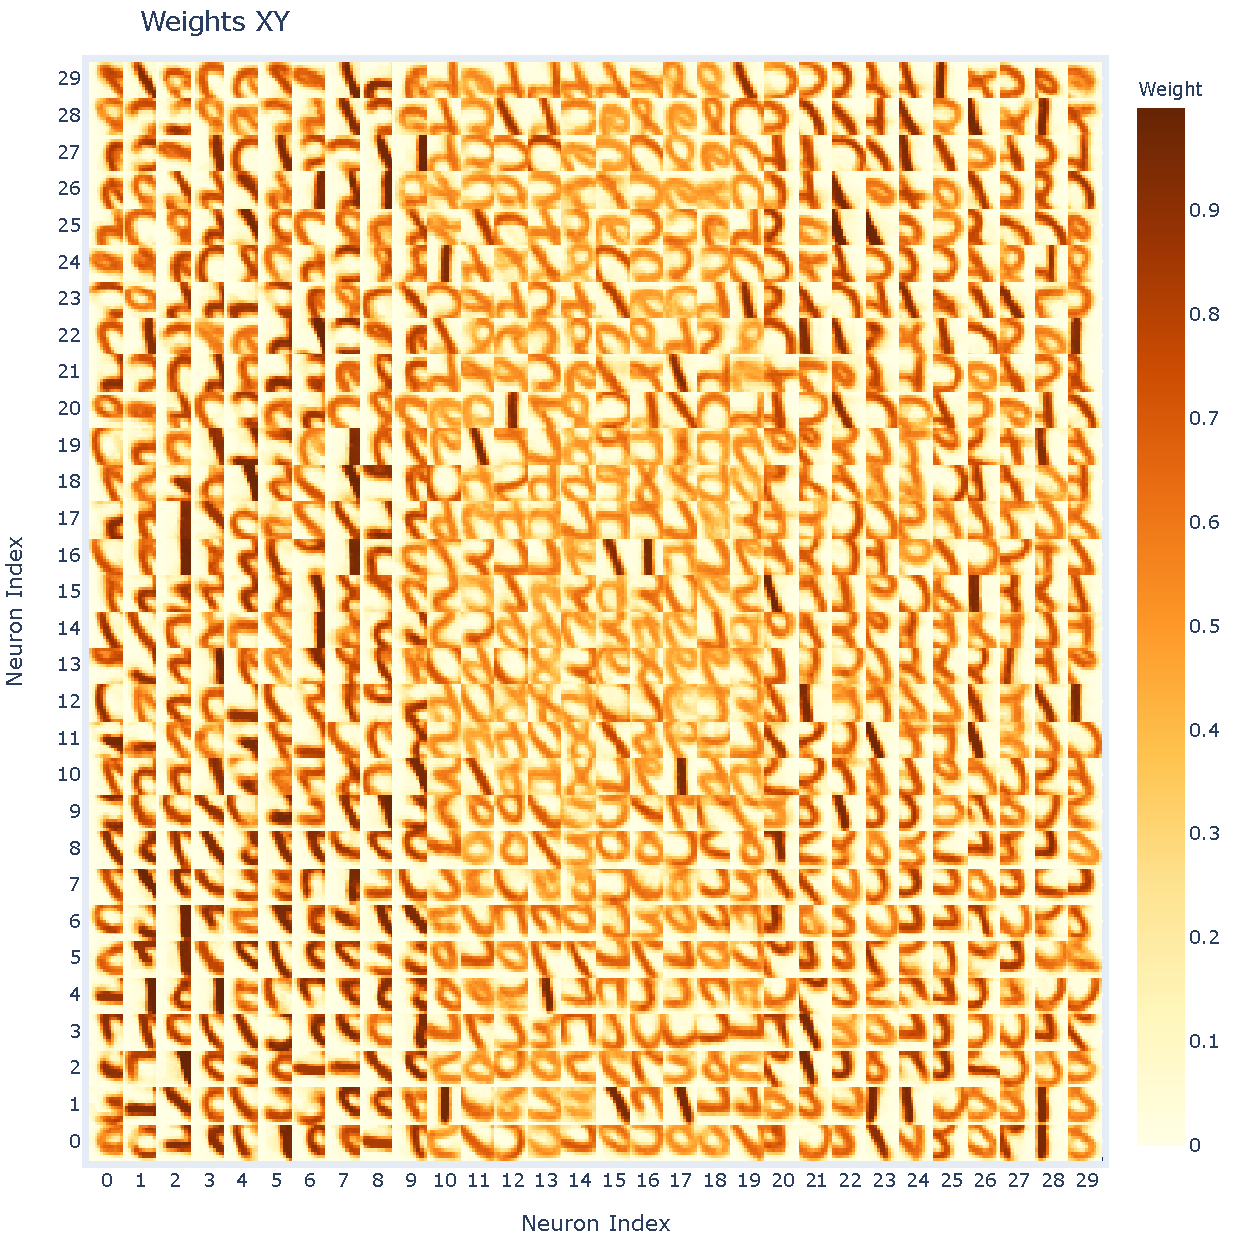
\includegraphics[width=\textwidth,keepaspectratio=true]{weights_XY.pdf}
    \caption{} 
    \label{fig:training:after_training}
\end{subfigure}
\caption{Visualization of $XY$ connection weights of a 900 $Y$ neurons (100 neurons for each of the 9 patches) network --- a 360 $ \times $ 360 matrix. The weights of one neuron correspond to a 12 $\times$ 12 square. The weights of the $Y$ neurons are grouped by patch - the lower left 120 $  \times $ 120 square  (10 $ \times $ 10 neurons) corresponds to the lower left patch, the center square corresponds to the center patch, and so on. Weights are initialized randomly (Fig. \ref{fig:training:before_training}), and after 1000 training iterations (Fig. \ref{fig:training:after_training}) the neurons learn different features, resembling digits elements}
\label{fig:training}
\end{figure}

\subsection{Spiking neural network activity interpretaion}

Several methods were used to interpret the activity of neurons in the $Y$ layer (that is, to correlate their activity with a certain class of recognizable digits): \textbf{patch voting}, \textbf{global voting}, \textbf{preselection by spikes voting} or a \textbf{linear classifier}. The first three methods have the advantage of being simple. However, the linear classifier significantly outperforms them in performance. \\

For the first three methods, it is necessary to calibrate the <<votes>> of neurons. Each neuron of the $Y$ layer is assigned 10 numbers (votes) for each digits class (from 0 to 9). The neuron-digit vote is calculated as the average number of spikes produced by the neuron in responce to the observation of this digit images by the network (throughout the entire time of the simulation) ---
$$ vote_i = \frac{\sum_ {1}^{n_{i}}{\sum_{0}^{t_{max}} s_t}} {n_{i}} \text {,} $$
where $ s_t $ takes the value 0 or 1 depending on the presence of a spike at a given time, $ n_i $ is the size of the calibration sample for the digit $ i $ (we used $ n_i = 1000 $).

For all networks, this calibration process was used for 10,000 examples from a calibration sample especially selected from the test part of the MNIST dataset, as noted above. Note that calibration is nota  part of the network training, since it is only included in the algorithm for interpreting the behavior of the SNS. The votes are used as a measure of confidence of the neuron in each of the digits classes. The example votes are shown in Fig. \ref{fig:votes}.

\begin{figure}
\centering
\begin{subfigure}{\textwidth}
    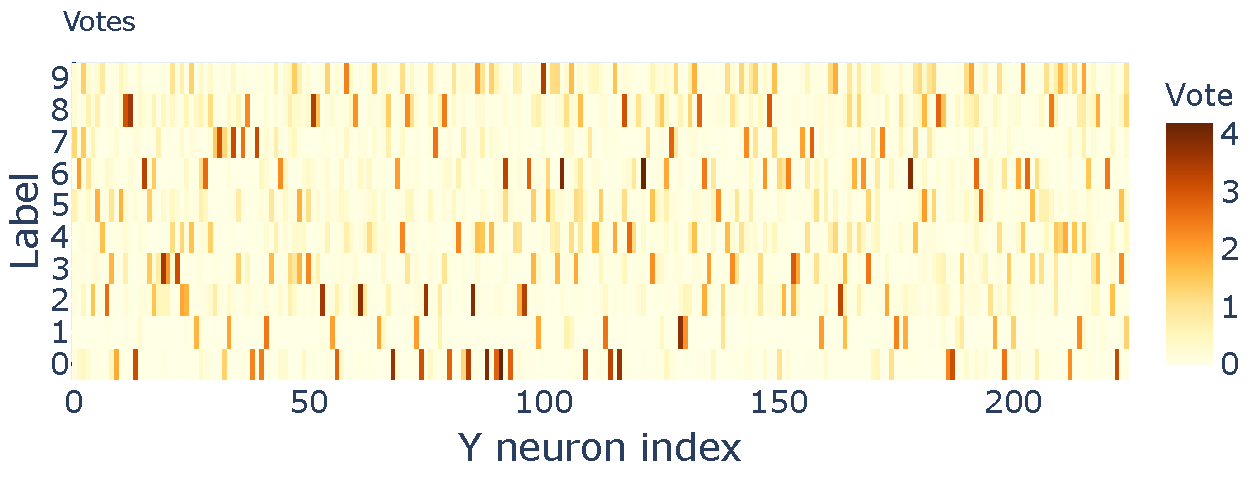
\includegraphics[width=\textwidth,keepaspectratio=true]{votes.pdf}
    \caption{}
    \label{fig:votes:votes}
\end{subfigure}
\begin{subfigure}{\textwidth} 
    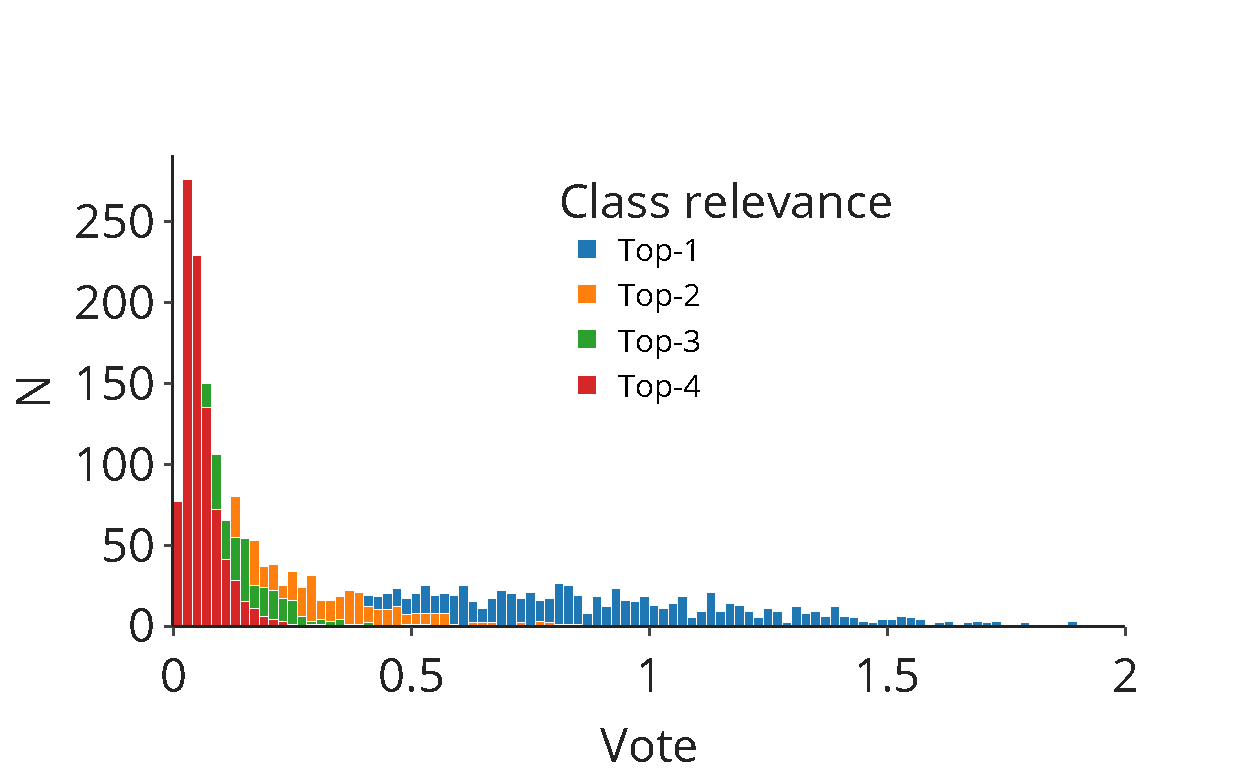
\includegraphics[width=\textwidth,keepaspectratio=true]{votes_distr_4.pdf} 
    \caption{}
    \label{fig:votes:distr}
\end{subfigure}
\caption{Votes visualization for a network with 225 $Y$ neurons. All $Y$ neurons votes are shown in Fig. \ref{fig:votes:votes}. High values correspond to a large specialization on the corresponding class. It can be seen that almost all neurons have a nonzero vote value, therefore, almost all neurons in the network are active. Votes distrivution for the 4 most relevant classes (for each neuron) are shown in Fig. \ref{fig:votes:distr}. It can be seen that the vote value (average number of spikes per class) drops significantly with relevance decreasing}
\label{fig:votes}
\end{figure}

Further, the product of the number of neuron spikes by its vote will be called \textit{score}.

In \textbf{global voting}, the network's response is considered to be the class with the highest \textit{score} among all neurons.

In \textbf{patch voting} the network response is considered to be the class with the highest \textit{score} among neurons with the highest \textit{score} per patch --- similiar to a maxpool operation in ANNs.

\textbf{Preselection by spikes voting} is done in a similiar fassion, but comparing the number of spikes, not \textit{scores}.

When using a \textbf{linear classifier}, the sums of spikes of individual  $ Y $ layer neurons are fed as features to te classifier, which is trained to predict the true image labels. As in other methods of interpreting the network activity, classifier training is performed on a separate calibration sample.

To evaluate the interpretation algorithm, accuracy is used - the ratio of the number of correctly recognized objects from a test sample to the size of the test sample. In this work, the test sample size (when measuring the accuracy for individual networks) is 10,000.

Accuracy learning curves (Fig. \ref{fig:learning_curves}) were built for various interpretation algorithms. The accuracy was measured every 250 training iterations. To calibrate the interpretation algorithm at each step a calibration sample of 5000 was used, while to measure the accuracy, a test sample of 1000 was used.

After several thousand training iterations, the accuracy reaches a plateau. It is also noticeable that the three voting methods have very similar accuracy, while the linear classifier performes significantly better. The accuracy of even an untrained network can reach 70\% due to the fact that even with random weights initialization, different feature maps are formed, with some being a little better at recognizing certain patters, which can be amplified by the interpretaion alrorithm. It is known from \parencite{saunders2019locally} that for a sufficiently large number of parameters, a locally connected network outperforms a convolutional and fully connected network in learning speed, since more parameters are updated with each training iteration (at least one neuron per patch is active). In the present study, no such effect is observed, since the presented learning curves are constructed for insufficiently large networks. Interestingly, the use of a linear classifier does not improve the recognition accuracy for a fully connected network - most likely due to the selection of voting features throughout the image, in contrast to convolutional and locally connected architectures.

The linear classifier surpasses the LCSNN- and CSNN-based voting algorithms in accuracy, since it is a generalization of voting in the sense that it also uses the sum of the products of weights/votes by neurons activity. However, when training a linear classifier effective optimization algorithms (including gradient) are being used, while when voting we achieve practically the same goal (calculating satisfactory votes/weights) with a heuristic - the averaged activity of neurons by classes.

\begin{figure}
\centering
\begin{subfigure}{0.48\textwidth}
    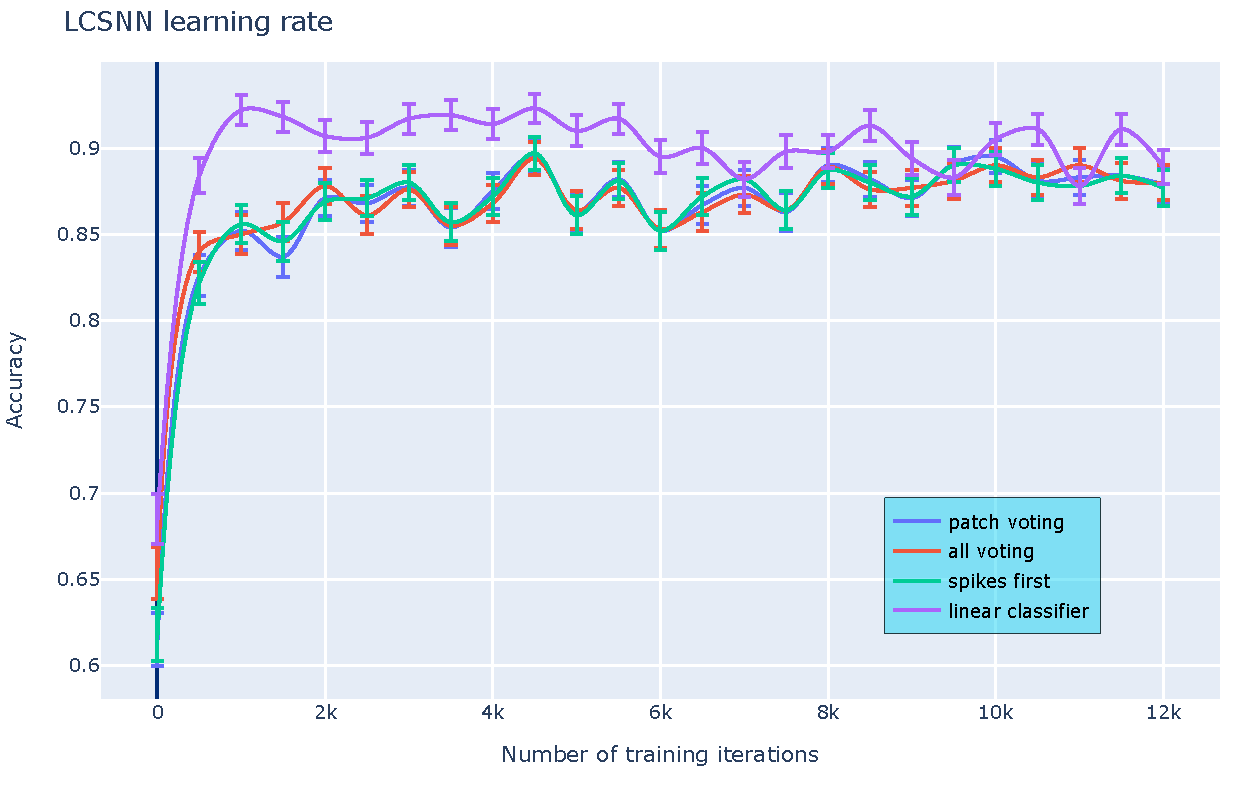
\includegraphics[width=\textwidth,keepaspectratio=true]{LCSNN_learning_rate.pdf}
 \caption{}
 \label{LCSNN_learning_curve}
\end{subfigure} 
\begin{subfigure}{0.48\textwidth} 
    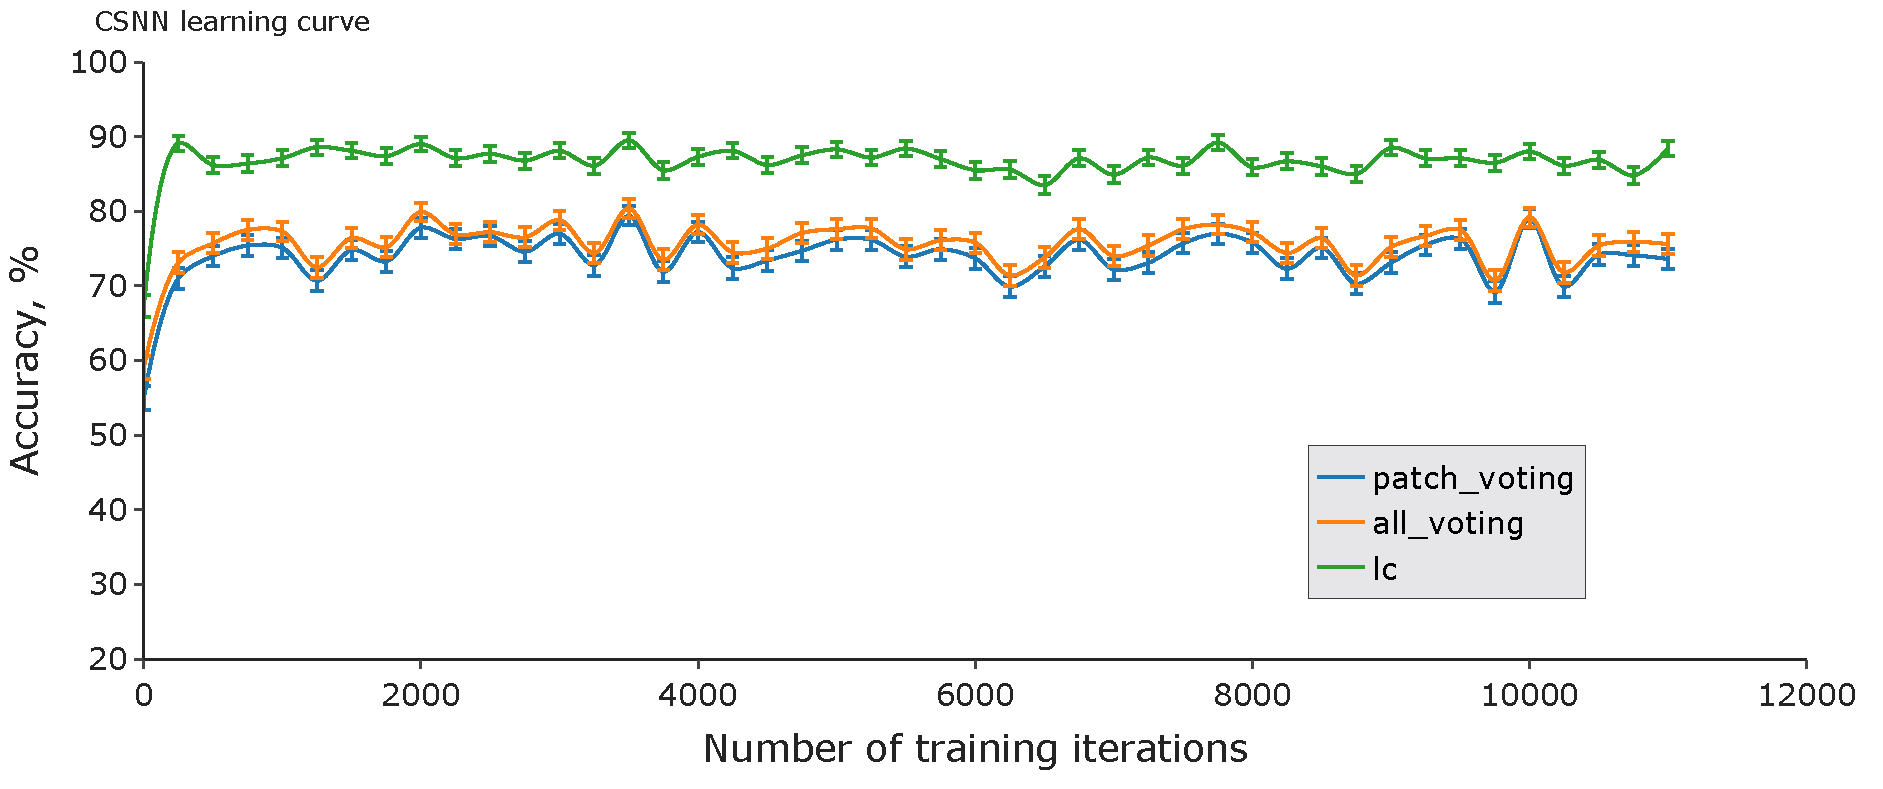
\includegraphics[width=\textwidth,keepaspectratio=true]{CSNN_learning_rate.pdf}
 \caption{}
 \label{CSNN_learning_curve}
\end{subfigure} 
\end{figure}
\begin{figure}\ContinuedFloat
\begin{subfigure}{0.48\textwidth} 
    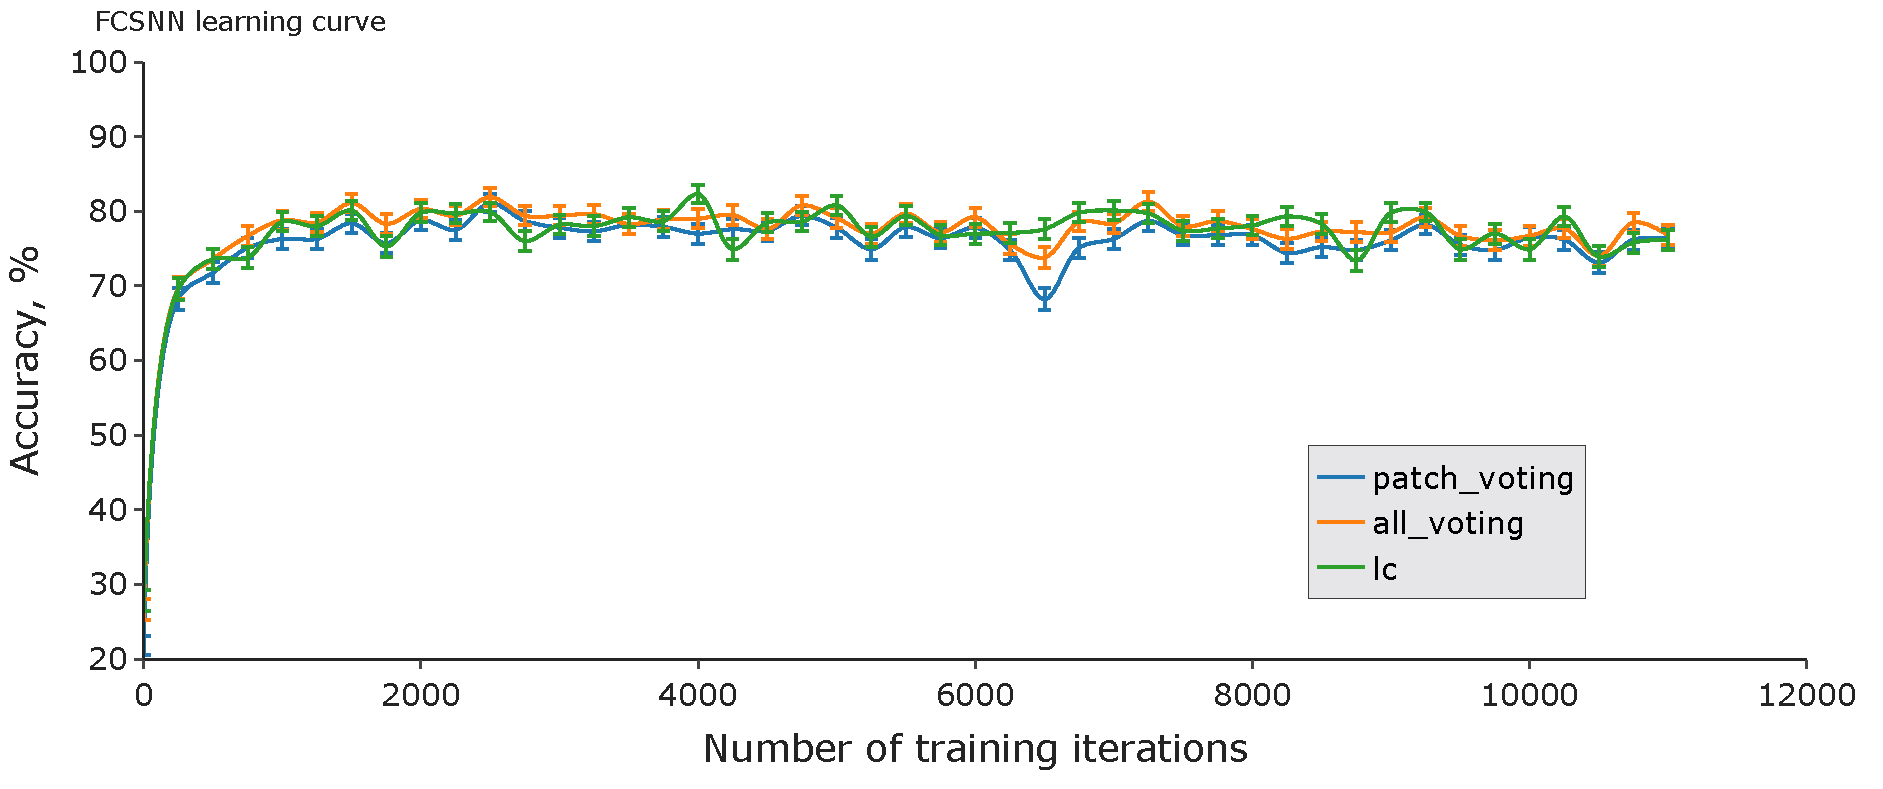
\includegraphics[width=\textwidth,keepaspectratio=true]{FCSNN_learning_rate.pdf}
 \caption{}
 \label{FCSNN_learning_curve}
\end{subfigure}
\caption{Comparison of learning curves of different architectures of SNNs with competition: (Fig. \ref{LCSNN_learning_curve}) LCSNN, (Fig. \ref{CSNN_learning_curve}) CSNN, (Fig. \ref{FCSNN_learning_curve}) FCSNN. The results are evaluated with different algorithms for the interpretation of activity. The \textbf{preselections by spikes} algorithm was only checked for LCSNN, because it achieves practically same results as \textbf{patch voting}. Standard deviations are plotted as errors. The networks have 100 channels (for a FCSNN the channel consists of a single neuron), the convolution kernel size ($k$) for the LCSNN is 12, and 8 for the CSNN}
\label{fig:learning_curves}
\end{figure}

\subsection{Comparison of convolution and local connections effectiveness}
Experiments were carried out to measure the accuracy of networks with different architectures. For convolutional and fully connected networks,  inhibitory connections similar to LCSNN were introduced. Note that using a linear classifier as an interpretation algorithm, it was possible to achieve 95\% accuracy for a locally connected network of 1000 channels with kernel size of 12.

\begin{table}
 \caption{Comparison of different architectures. For each configuration, the accuracy was measured $ N = 5 $ times. The table shows the arithmetic mean of the accuracy and its standard deviation. The <<kernel>> corresponds to the number $ k $ in the size of the convolution $ k \times k $}
\begin{center}
\begin{tabular}{|l|l|l|l|l|l|p{2.2cm}|p{2.2cm}|}
\hline
&\multicolumn{5}{c|}{Conviguration} & \multicolumn{2}{c|}{Accuracy, \%}\\
\hline
N & Architecture & Channels & Kernel & Parameters & $Y$ neurons & {Method \footnotemark[1]} & {Method \footnotemark[2]} \\
\hline\hline
{\textbf{1}} & {\textbf{LCSNN}} & {\textbf{1000}} & {\textbf{12}} & {\textbf{10287000}} & {\textbf{9000}} & {$\mathbf{92.3 \pm 0.7}$} & {$\mathbf{95.1 \pm 0.5}$}\\
\hline
2 & {LCSNN} & {100} & {12} & {218700} & {900} & {$87.5 \pm 0.9$} & {$91.5 \pm 0.6$}\\
\hline
3 & {LCSNN} & {100} & {8} & {260800} & {1600} & {$82.9 \pm 0.6$} & {$88.1 \pm 0.7$}\\
\hline
{\textbf{4}} & {\textbf{LCSNN\footnotemark[3]}} & {\textbf{25}} & {\textbf{12}} & {\textbf{37800}} & {\textbf{225}} & {$\mathbf{82.3 \pm 1.0}$} & {$\mathbf{88.2 \pm 0.6}$}\\
\hline
5 & {LCSNN} & {25} & {12} & {37800} & {225} & {$80.1 \pm 1.0$} & {$85.5 \pm 0.8$}\\
\hline
6 & {LCSNN} & {25} & {8} & {35200} & {400} & {$73.6 \pm 1.0$} & {$80.3 \pm 0.7$}\\
\hline\hline
7 & {CSNN} & {169} & {12} & {279864} & {1521} & {$79.2 \pm 1.6$} & {$85.7 \pm 1.4$}\\
\hline
8 & {CSNN} & {81} & {12} & {69984} & {729} & {$77.2 \pm 1.7$} & {$83.1 \pm 1.2$}\\
\hline
9 & {CSNN} & {100} & {8} & {164800} & {1600} & {$77.4 \pm 1.9$} & {$82.1 \pm 1.3$}\\
\hline
10 & {CSNN} & {25} & {12} & {9000} & {225} & {$65.8 \pm 0.7$} & {$77.1 \pm 0.6$}\\
\hline
11 & {CSNN} & {25} & {8} & {11200} & {400} & {$63.1 \pm 1.2$} & {$75.8 \pm 0.5$}\\
\hline\hline
12 & {FCSNN} & {100} & {20} & {49900} & {100} & {$81.4 \pm 0.9$} & {$82.1 \pm 0.8$}\\
\hline
\end{tabular}
\end{center}
 \label{results}
\end{table}

\footnotetext[1]{Best voting algorithm}
\footnotetext[2]{Linear classifier}
\footnotetext[3]{Network with trainable inhibitory connections}

It can be seen (№2 and №7 in the \ref{results} table) that the locally connected network surpasses the convolutional network in accuracy even if the number of parameters of the latter is slightly larger. Also, having too small convolution kernel size leads to lower network accuracy, because it leads to learning of less essential features. Indeed, in traditional deep learning based, either shallow networks with large convolution kernels are used, or deep networks with small convolution kernels.

It should be noted that SNNs can achieve significantly higher recognition accuracy on MNIST. It can be achieved by: (i) networks with a significantly larger number of parameters (for example, with an increased number of channels); (ii) deeper networks; (iii) more efficient learning algorithms (for example, supervised learning or using the contrastive loss function \parencite{contrastive_loss}). At the same time, achieving the highest possible accuracy was not the goal of this study, which is primarily aimed at comparing various SNN architectures.

\begin{table}
 \caption{Results from other studies of spiking neural networks with MNIST}
\begin{center}
\begin{tabular}{|l|p{4cm}|p{7cm}|l|l|}
\hline
Paper & Architecture & Training & Accuracy, \% \\
\hline\hline
{This study} & {Local + competition} & {Unsupervised} & {$95.1 \pm 0.5$}\\
\hline\hline
{\parencite{saunders2019locally}} & {Local + competition} & {Unsupervised} & {$95.07 \pm 0.63$}\\
\hline
{\parencite{mnist2}} & {Fully connected + competition} & {Unsupervised} & {95}\\
\hline
{\parencite{MaxActiv1}} & {Fully connected + competition} & {Supervised / Semi-supervised} & {95.4 / 72.1}\\
\hline
{\parencite{conv1}} & {Convolutional} & {Semi-supervised} & {$96.95 \pm 0.08$}\\
\hline
{\parencite{conv2}} & {Convolutional} & {Semi-supervised} & {$99.28 \pm 0.10$}\\
\hline
{\parencite{conv3}} & {Convolutional} & {Semi-supervised} & {$97.20 \pm 0.07$}\\
\hline
\end{tabular}
\end{center}
\end{table}

\pagebreak

\section{Inhibitory connections training}
\label{section:competition-training}
The result obtained in this work are comparable to the result of \parencite{saunders2019locally}. Note that the results achieved with unsupervised training are only slightly inferior to the results achived by supervised training. Note, that our best locally connected network with trainable competitions had $ 10^7 $ parameters (of which $ 1 \cdot 10^6 $ are forward connections and $ 9 \cdot 10^6 $ inhibitory connections), which is less than $ 4.6 \cdot 10^7 $ (of which $ 0.5 \cdot 10^7 $ forward conenctions and $ 4.1 \cdot 10^7 $ compettition connections) for a fully connected network with competition from \parencite{mnist2}. In addition, the network from \parencite{mnist2} was trained for $ 1 \cdot 10^6 $ iterations, while in this study the number of training iterations did not exceed 5000. 

\section {Inhibitory connections training}
Inhibitory connections $YY$ greatly affect the training of forward connections $XY$. Large absolute values of inhibitory weights contibute to greater variability and specialization in training $Y$ neurons, as for each receptive field similar weights $XY$ neoruns are simultaneously active (Fig. \ref{fig:high_comp}). On the contrary, inhibitory weights of small absolute values do not allow neurons to specialize effectively (Fig. \ref{fig:high_comp}). 

\begin{figure}
\centering
\begin{subfigure}{0.45\textwidth}
    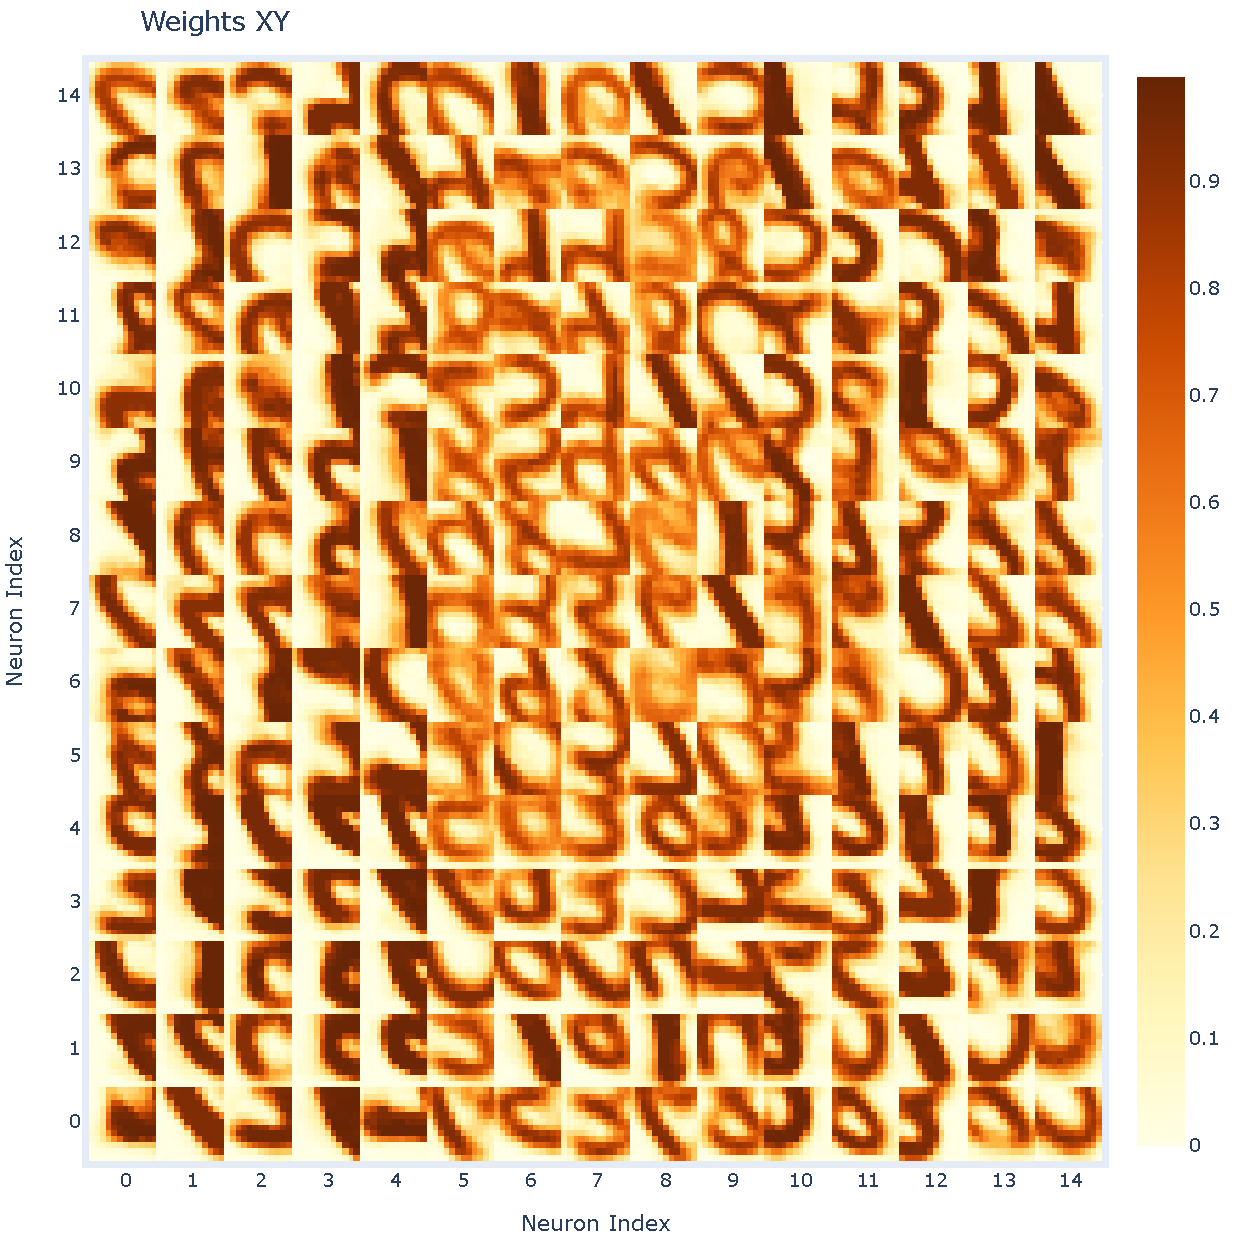
\includegraphics[width=\textwidth,keepaspectratio=true]{weights_XY_good.pdf}
    \caption{}
    \label{fig:competition_effect_on_training:high_comp}
\end{subfigure}
\begin{subfigure}{0.45\textwidth}
    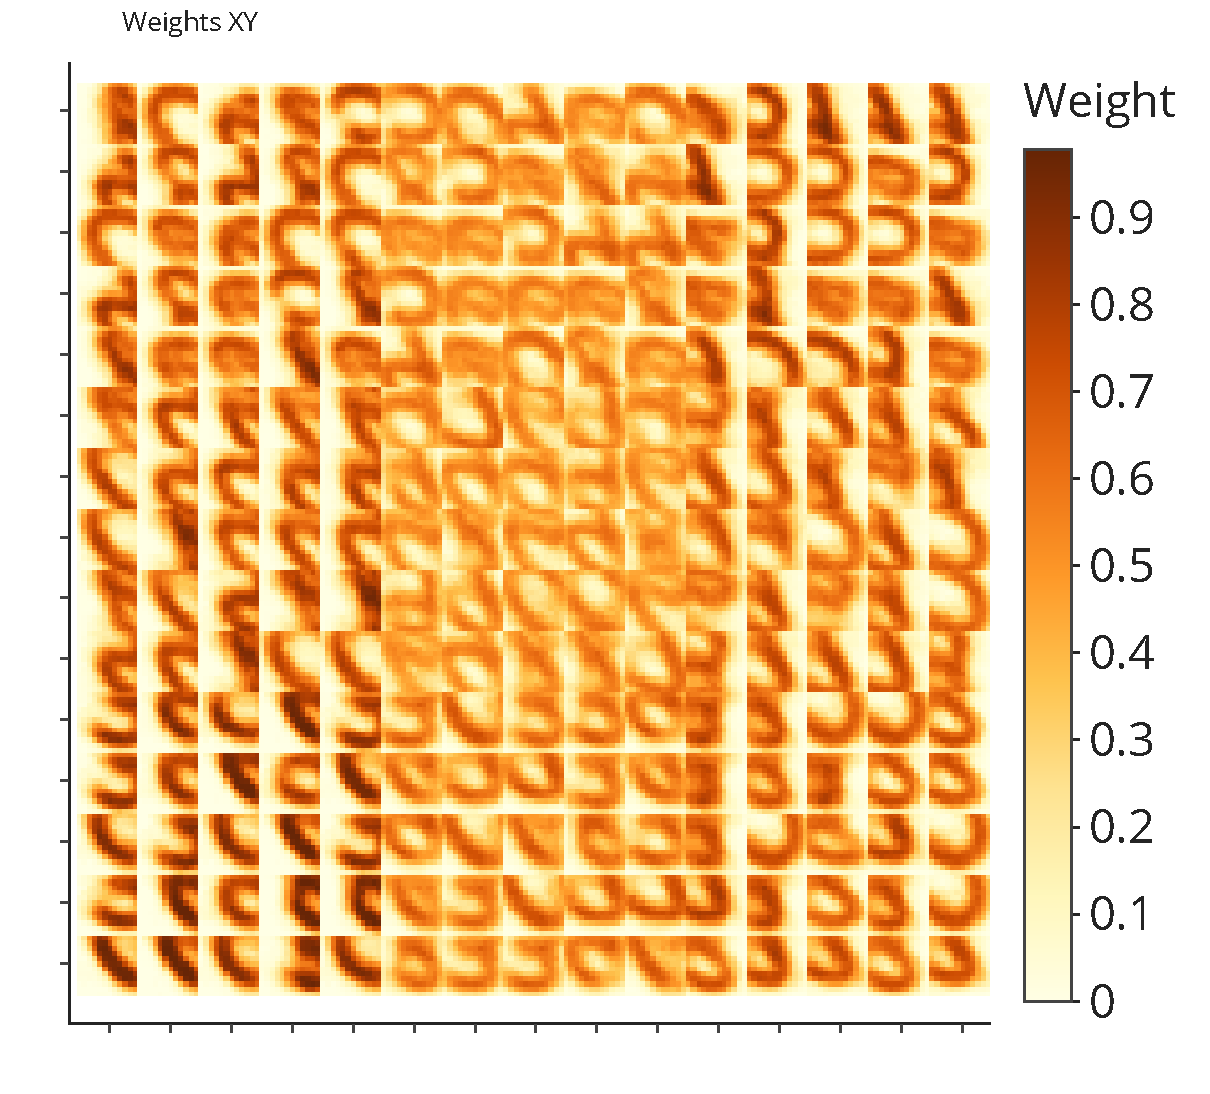
\includegraphics[width=\textwidth,keepaspectratio=true]{weights_XY_bad.pdf} 
    \caption{}
    \label{fig:competition_effect_on_training:low_comp}
\end{subfigure}
\caption{The effect of competition on $ XY $ connections training. Fig. \ref{fig:competition_effect_on_training:low_comp} shows poorly specialized neuros with similar features - the result of training with competiiton weights set to $-10$, while Fig. \ref{fig:competition_effect_on_training:high_comp} features highly specialized neurons with diverse features, trained with inhibitory weights set to $-100$}
\label{competition-training-importance}
\end{figure}

All SNNs discussed in this paper up to this point had fixed competition. In this regard, the question arised of how the trianing of inhibitory weights affects the accuracy of the network.

To answer this question, in order to update the $ YY $ connections, the anti-STDP rule was chosen (the rule opposite in the signs of $ A_{+} $ and $ A_{-} $ to standard STDP). For different values of the parameters of this rule, different distributions of inhibitory weights were obtained. The initial values of the weights were set from a uniform distibution from 0 to a certain negative values. Experiments were carried out with LCSNN networks.

\begin{table}
 \caption{anti-STDP parameters}
\begin{center}
\begin{tabular}{|l|l|l|l|l|}
\hline
Figure & {$\tau_{+}$, ms} & {$\tau_{-}$, ms} & {$A_{+}$} & {$A_{-}$} \\
\hline
\ref{fig:worst_competition_distribution} & 14.7 & 14.2 & -0.5 & -1.5 \\
\hline
\ref{fig:medium_bad_competition_distribution} & 5.4 & 15.1 & -1.2 & -0.6 \\
\hline
\ref{fig:medium_good_competition_distribution} & 17.6 & 24.5 & -1.9 & -1.6 \\
\hline
\ref{fig:best_competition_XY} & 17.7 & 16.5 & -0.1 & -1.6\\
\hline
\end{tabular}
\end{center}
\end{table}

\begin{figure}
\centering
\begin{subfigure}{0.45\textwidth}
    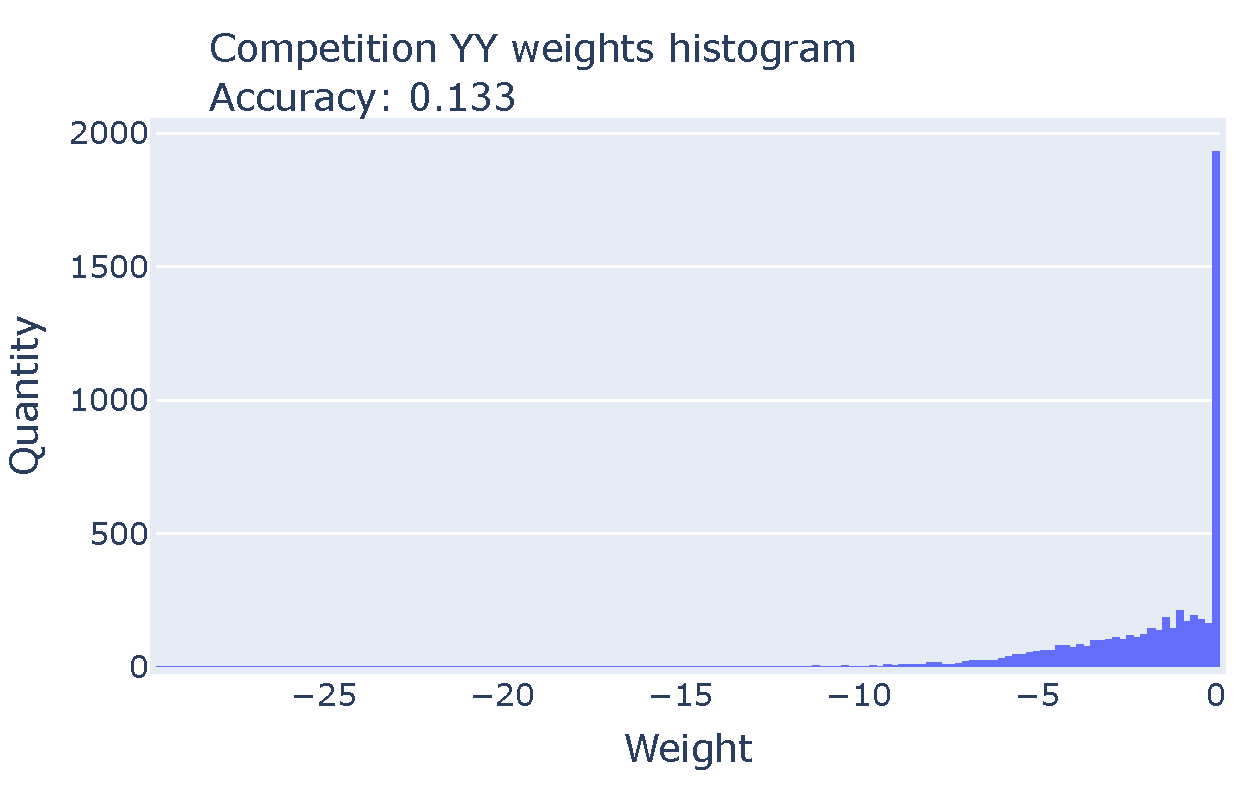
\includegraphics[width=\textwidth,keepaspectratio=true]{competition_distribution_worst.pdf}
    \caption{}
    \label{fig:competition_distributions:weakest}
\end{subfigure}
\begin{subfigure}{0.45\textwidth}
    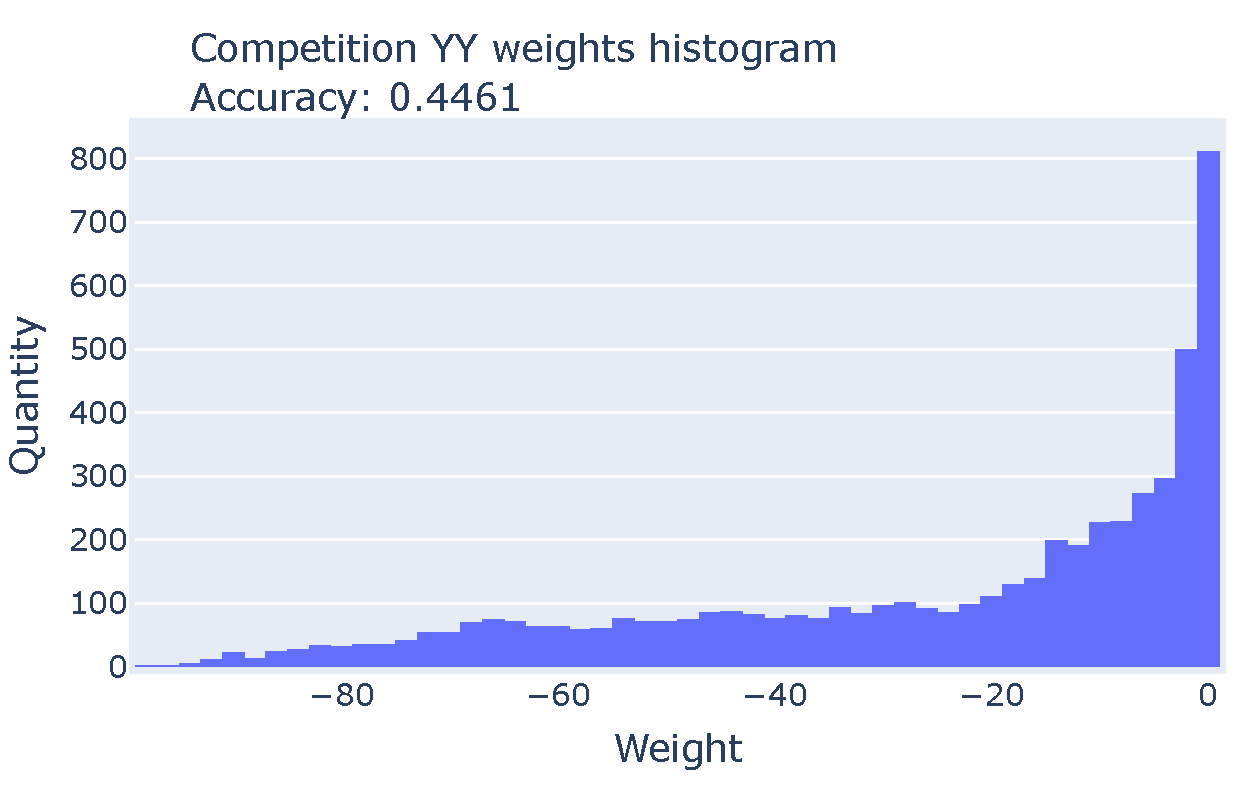
\includegraphics[width=\textwidth,keepaspectratio=true]{competition_distribution_medium_bad.pdf}
    \caption{}
    \label{fig:competition_distributions:weak}
\end{subfigure}
\\
\begin{subfigure}{0.45\textwidth}
    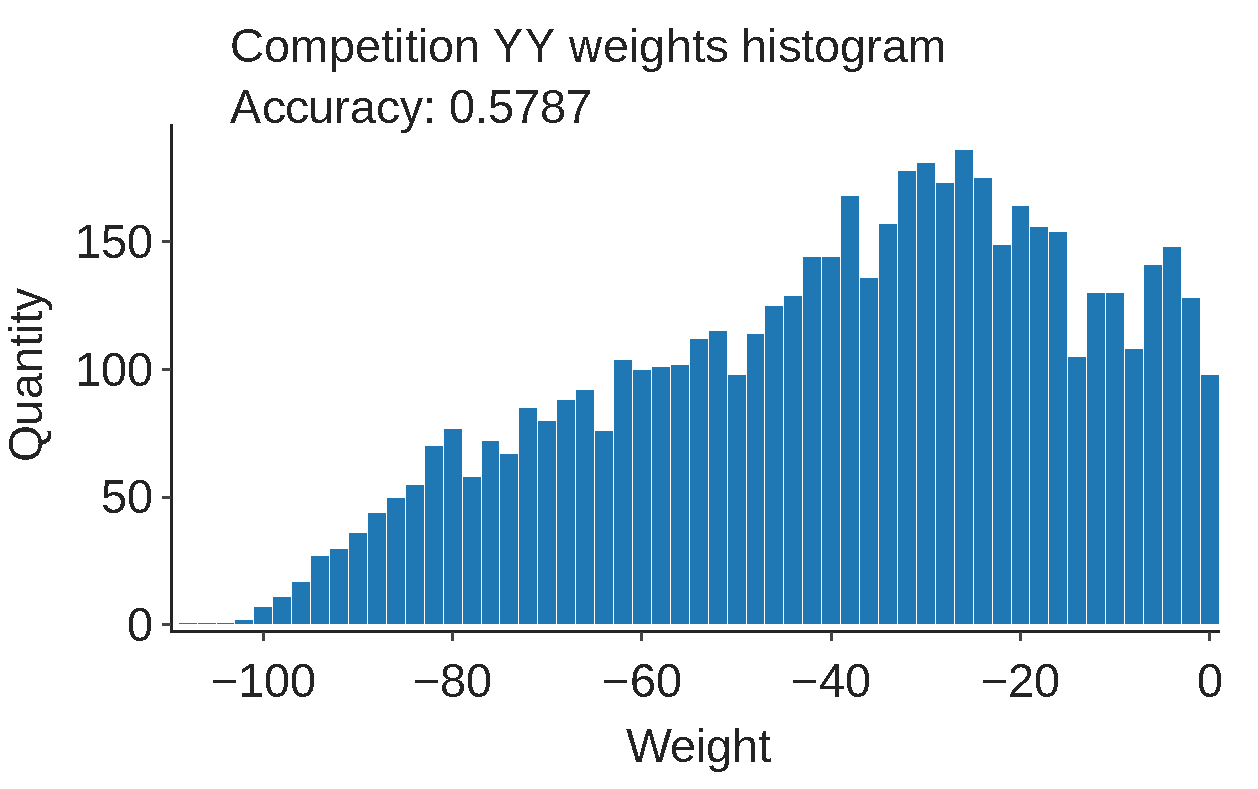
\includegraphics[width=\textwidth,keepaspectratio=true]{competition_distribution_medium_good.pdf}
    \caption{}
    \label{fig:competition_distributions:medium}
\end{subfigure}
\begin{subfigure}{0.45\textwidth}
    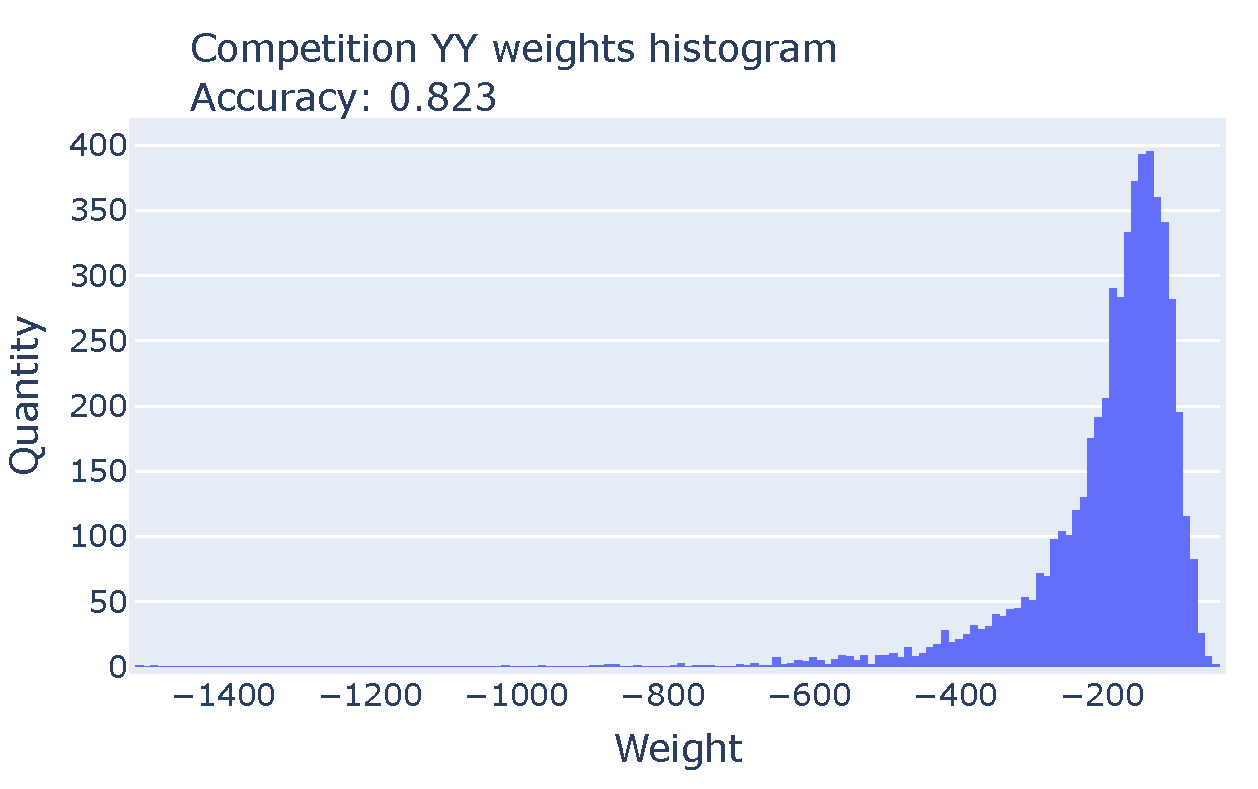
\includegraphics[width=\textwidth,keepaspectratio=true]{competition_distribution_best.pdf}
    \caption{}
    \label{fig:competition_distributions:strong}
\end{subfigure}
\caption{Different competition ($YY$) weights distributions: weakest competition (Fig. \ref{fig:competition_distributions:weakest}), weak competition (Fig. \ref{fig:competition_distributions:weak}), medium competition (Fig. \ref{fig:competition_distributions:medium}) and strong competition (Fig. \ref{fig:competition_distributions:strong})}
\label{fig:competition_distributions}
\end{figure}

It can be seen that the accuracy of the network increases when the distribution of inhibitory weights is shifted towards larger negative values. Note again that the goal was not to find the parameters that provide maximum accuracy, but to study the influence of competition training on the accuracy of the network with a given configuration of the remaining parameters.

It is noteworthy that not all $ YY $ connections end up with a large value (Fig. \ref{fig:competition_distributions:strong}). This is due to the fact that neurons specializing in substantially different features do not need competition, since they do not exhibit high activity at the same time.

\begin{figure}
\centering
\begin{subfigure}{0.45\textwidth} 
    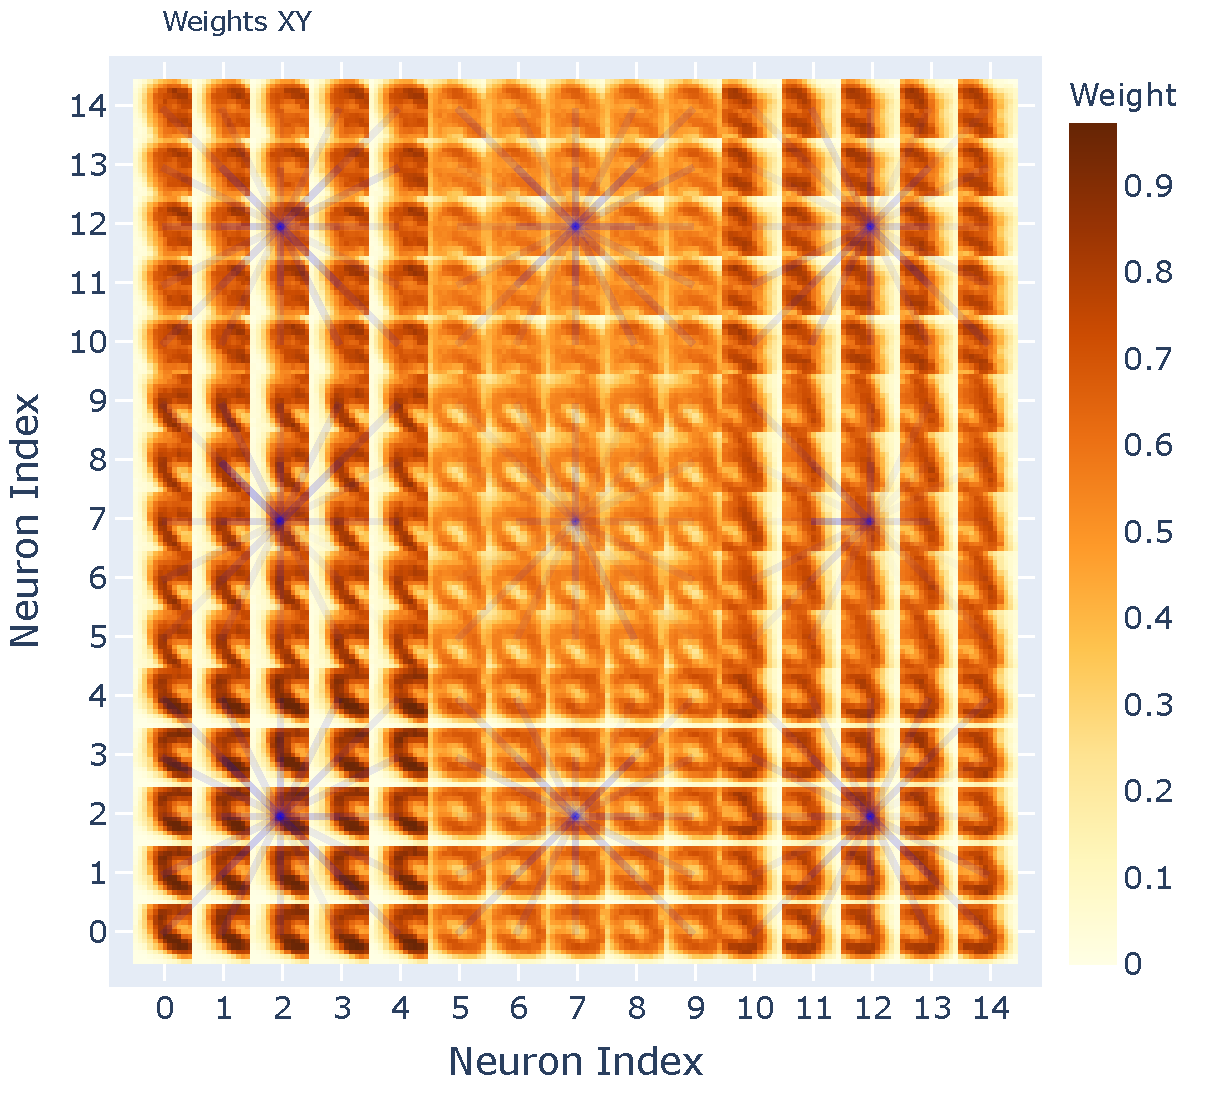
\includegraphics[width=\textwidth,keepaspectratio=true]{competition_on_XY_worst.pdf}
    \caption{}
    \label{fig:worst_competition_distribution}
\end{subfigure}
\begin{subfigure}{0.45\textwidth}
    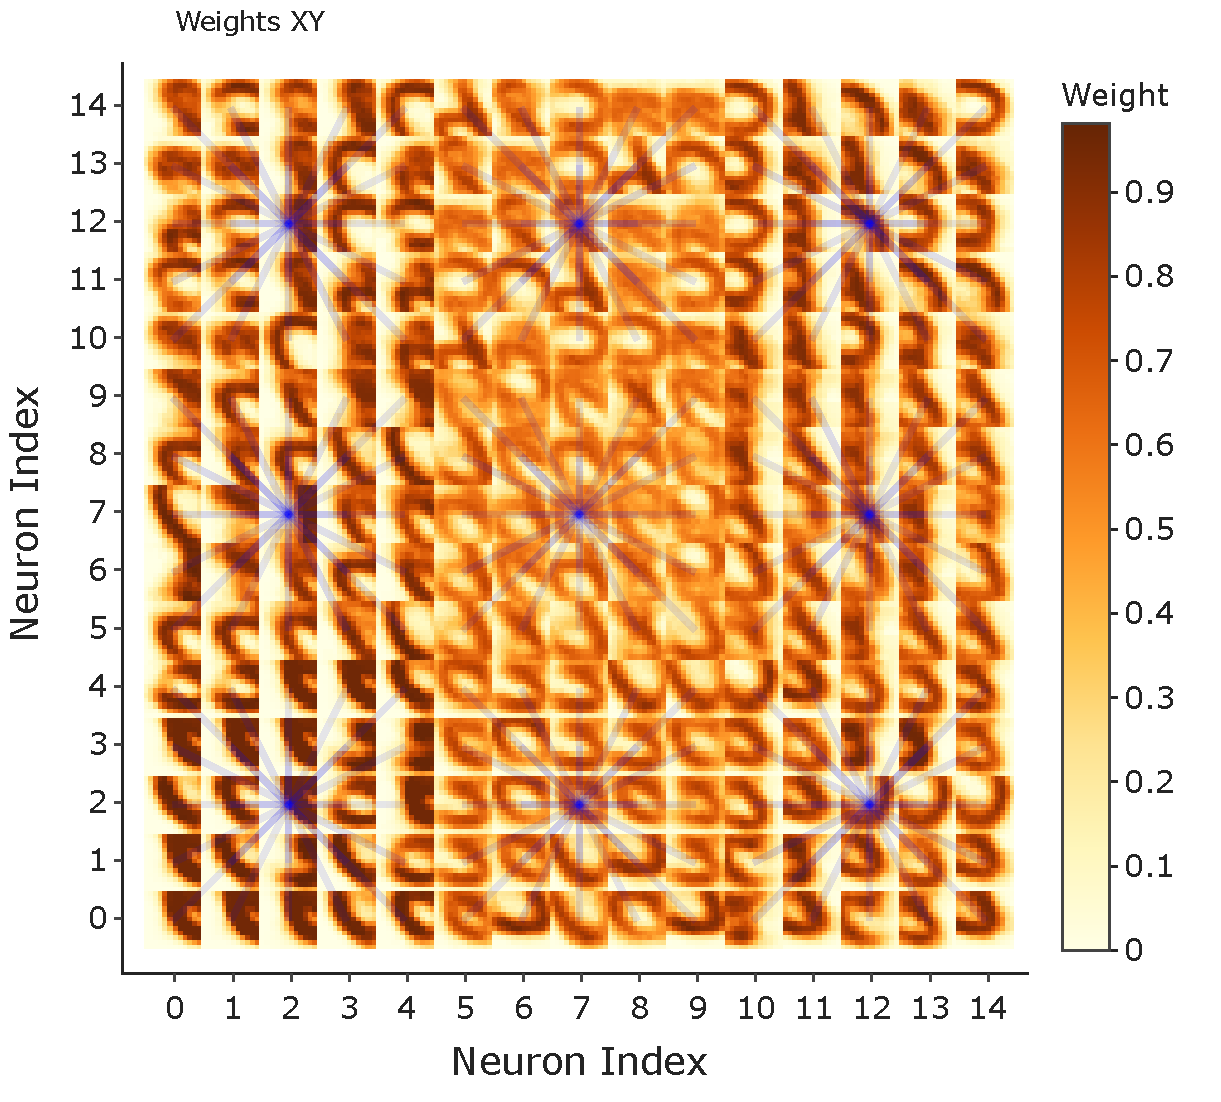
\includegraphics[width=\textwidth,keepaspectratio=true]{competition_on_XY_medium_bad.pdf}
    \caption{}
    \label{fig:medium_bad_competition_distribution}
\end{subfigure}
\\
\begin{subfigure}{0.45\textwidth}
    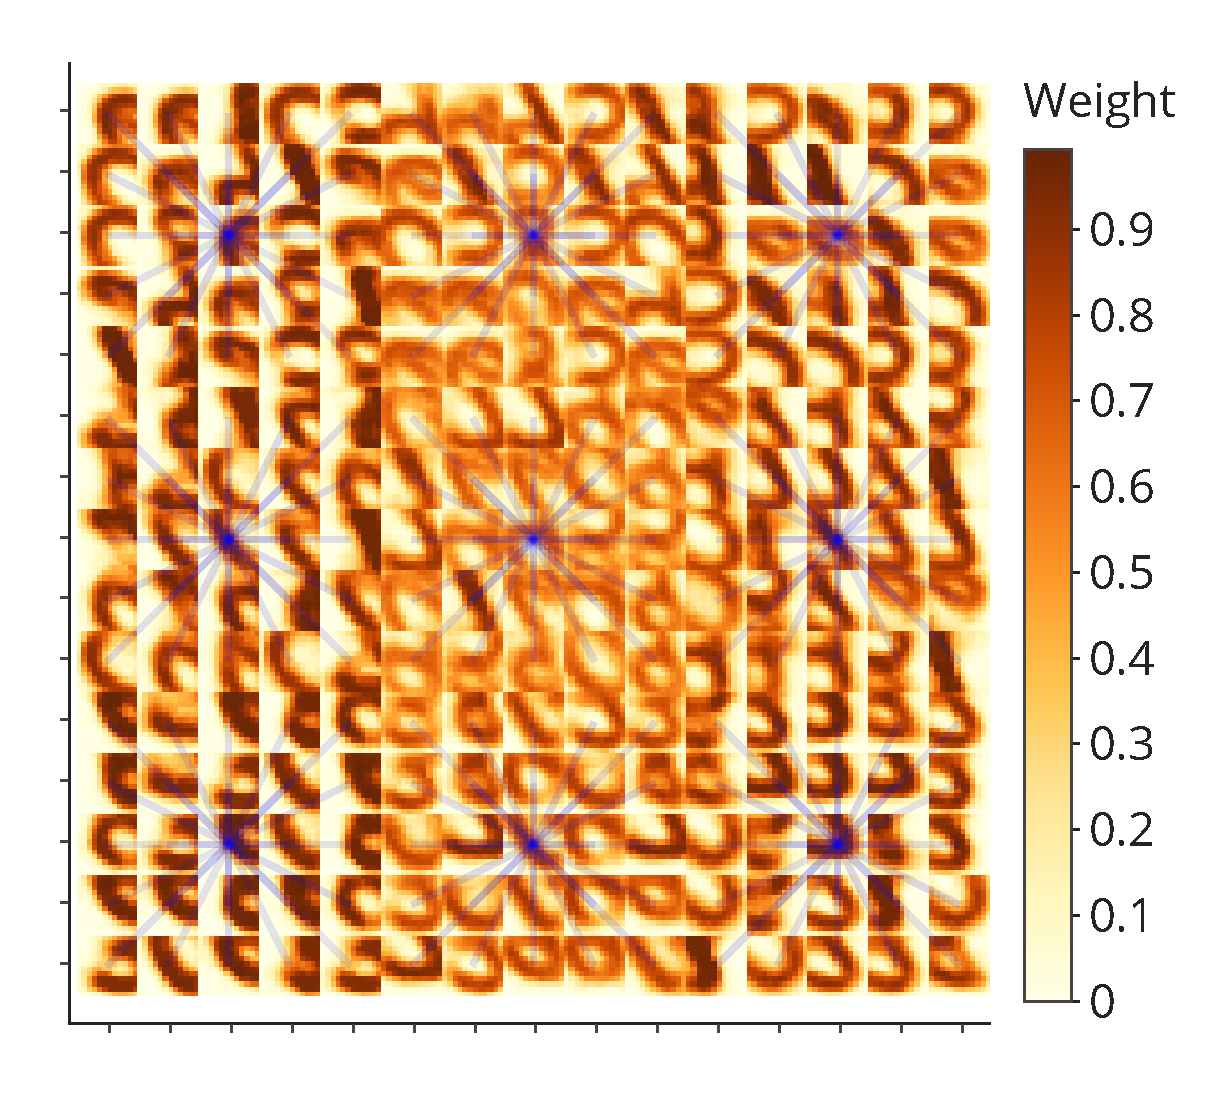
\includegraphics[width=\textwidth,keepaspectratio=true]{competition_on_XY_medium_good.pdf}
    \caption{}
    \label{fig:medium_good_competition_distribution}
\end{subfigure}
\begin{subfigure}{0.45\textwidth} 
    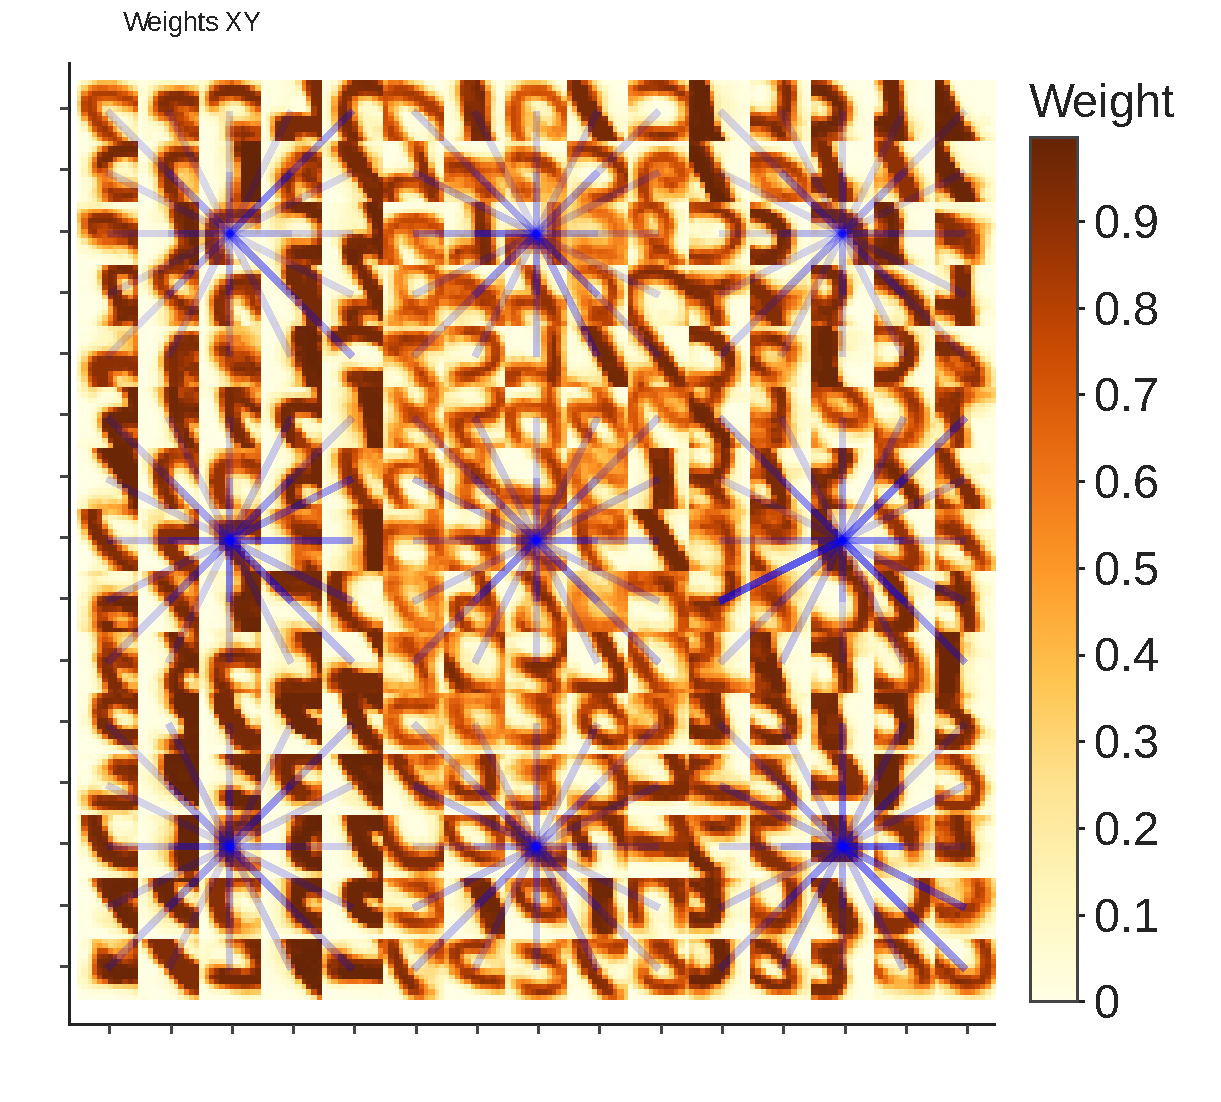
\includegraphics[width=\textwidth,keepaspectratio=true]{competition_on_XY_best.pdf}
    \caption{}
    \label{fig:best_competition_XY}
\end{subfigure}
\caption{Visualization of inhibitory weights on top of $ XY $ weights for the networks from Fig. (\ref{fig:competition_distributions}). Competition weights are shown only for one center neuron in each receptive field to avoid cluttering the visualization. The saturated blue color corresponds to the inhibitory weights of large absolute value (the arithmetic mean between the weights $ W_{ij} $ and $ W_{ji} $ is used). Figures \ref{fig:worst_competition_distribution}-\subref{fig:best_competition_XY} correspond to the same networks as Figures \ref{fig:competition_distributions:weakest}-\subref{fig:competition_distributions:strong} (from weakest to strongest competition). It can be seen that similar features have higher inhibitory connections weights than different}
\end{figure}

Competition training was carried out only on networks of 25 channels (225 neurons), since its simulation requires large computational resources.

During the optimization of the models, the accuracy of a large number of LCSNNs was measured with various hyperparameter configurations (Fig. \ref{fig:hyperparams}). It can be seen that configurations with high accuracy (dark lines) are localized in a manner that encourages negative weight accumulation for larger time differencies $t_{post} - t_{pre}$ between -post and -pre spikes (for the anti-STDP weight update rule). 

\begin{figure}
\begin{center}
 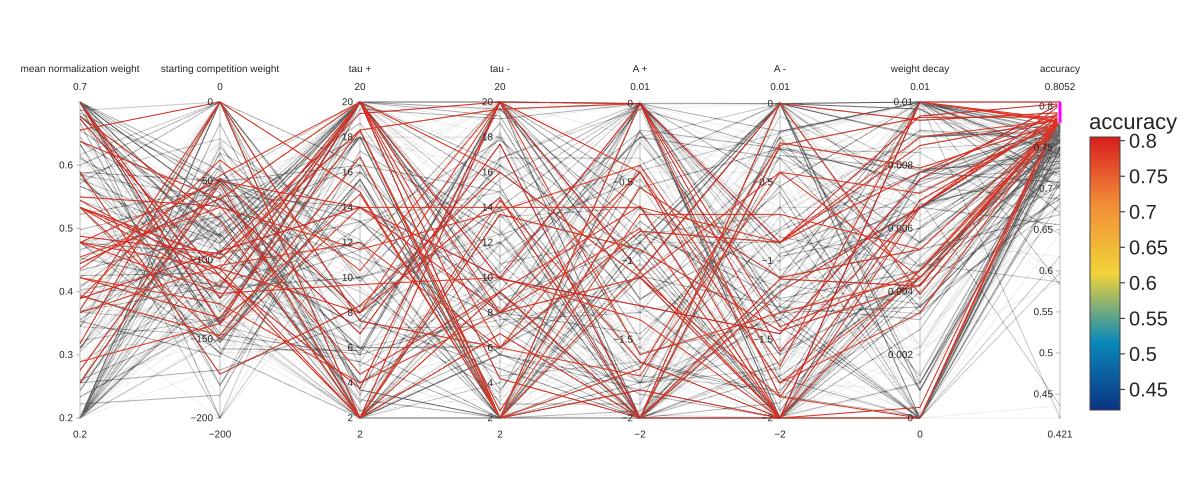
\includegraphics[,
 width=\textwidth,keepaspectratio=true]{hyperparams.png}
 
\caption{Visualization of the achieved LCSNN recognition accuracy when using various combinations in the hyperparameters space. The parameters <<normalization weight>>, <<initial competition weight>> and <<weight decay>> are responsible for the weights values, and the next two parameters are combinations of anti-STDP parameters
}
 \label{fig:hyperparams} 
\end{center} 

\end{figure}

\subsection{Trained inhibitory weights analysis}

In addition, inhibitory weights clamping (during training) experiments were carried out. It turned out that the inhibitory weights in the entire range of their variation are important for the effective LCSNN functioning, since both the upper and lower clamps negatively affect the classification accuracy (Fig. \ref{fig:compe_clamp}). This is due to the fact that high competition contributes to greater specialization of neurons and therefore is useful, and low competition allows neurons to cooperate and recognize digits together (including ensuring the accumulation of more statistics for calibrating the voices of neurons).

\begin{figure}
\centering 
\begin{subfigure}{0.45\textwidth}
    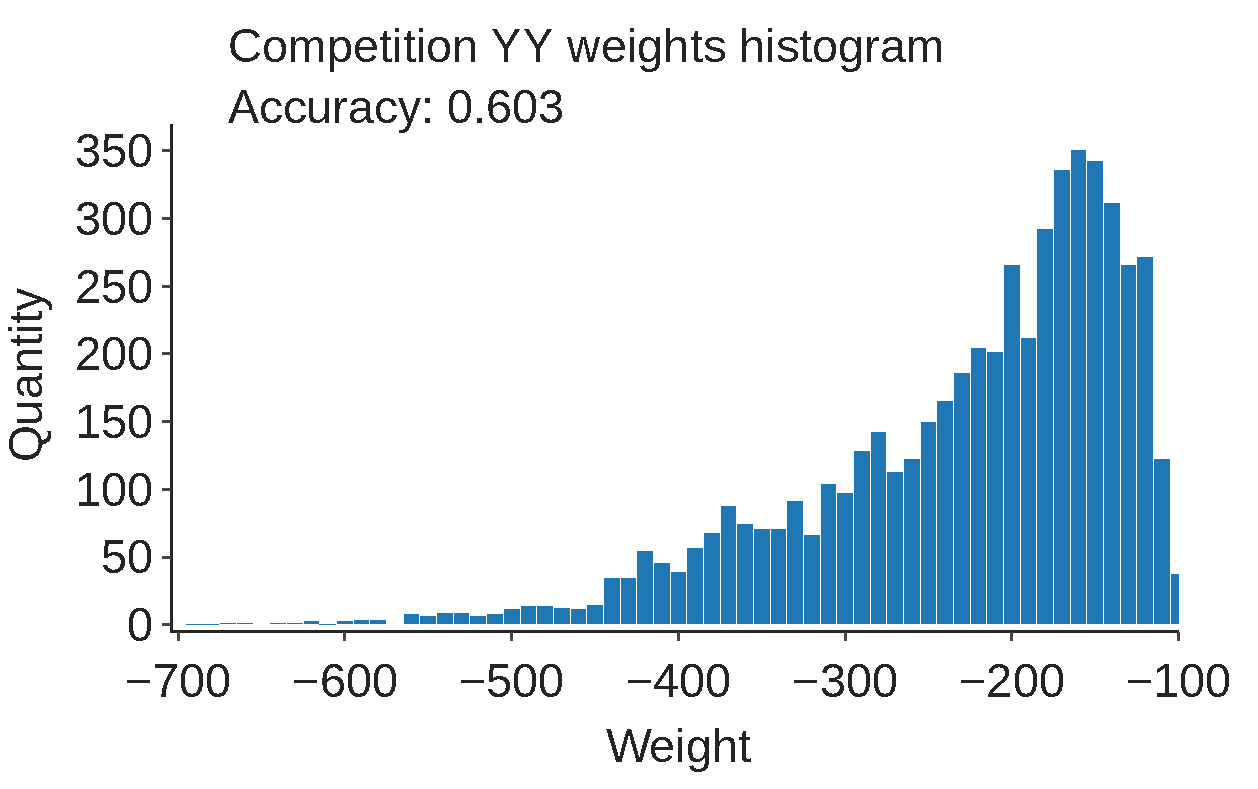
\includegraphics[width=\textwidth,keepaspectratio=true]{competition_distribution_clamp_low.pdf}
    \caption{}
    \label{fig:compe_clamp:low_distr}
\end{subfigure}
\begin{subfigure}{0.45\textwidth}
    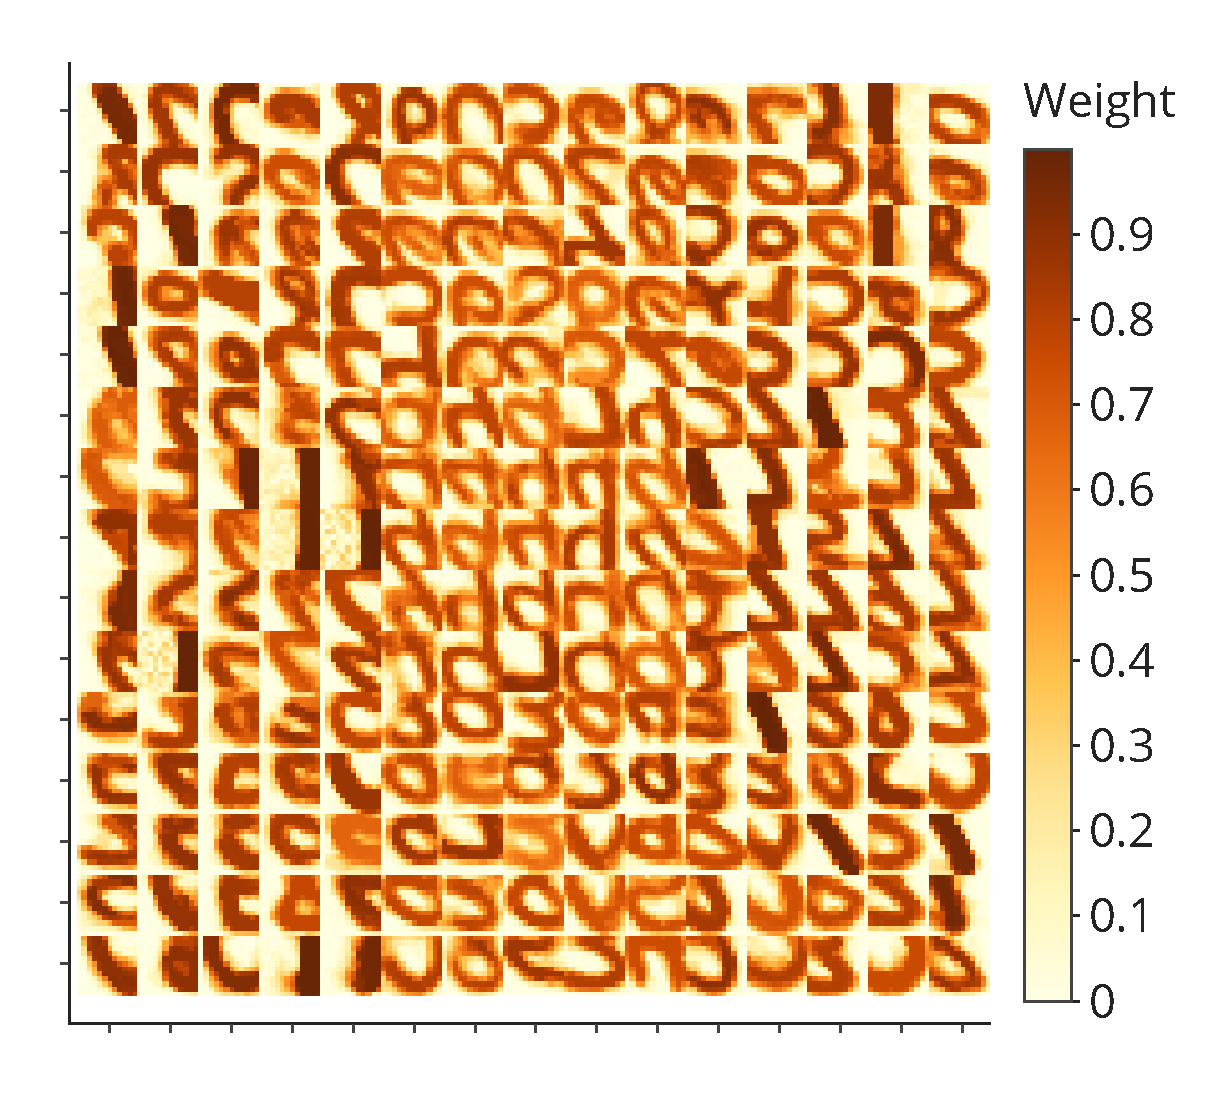
\includegraphics[width=\textwidth,keepaspectratio=true]{weights_XY_clamp_low.pdf}
    \caption{}
    \label{fig:compe_clamp:low_weights}
\end{subfigure} 
\begin{subfigure}{0.45\textwidth}
    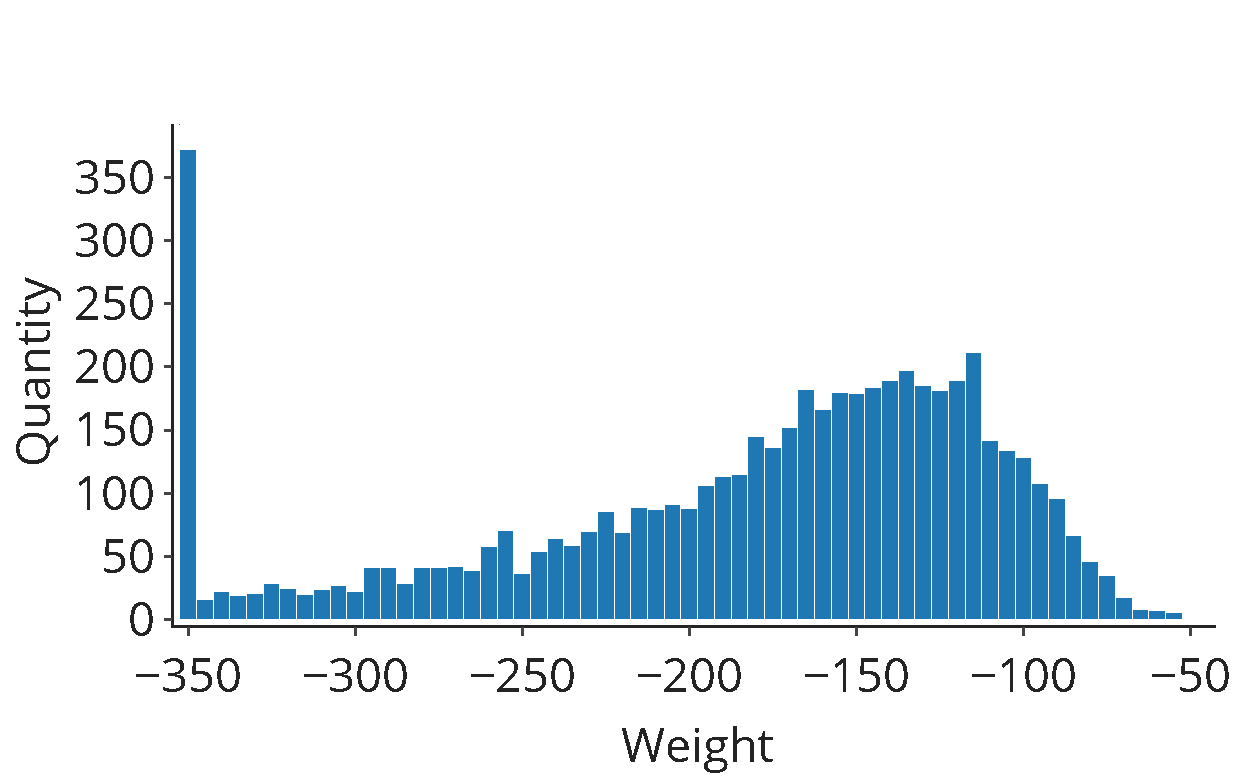
\includegraphics[width=\textwidth,keepaspectratio=true]{competition_distribution_clamp_high.pdf}
    \caption{}
    \label{fig:compe_clamp:high_distr}
\end{subfigure}
\begin{subfigure}{0.45\textwidth} 
    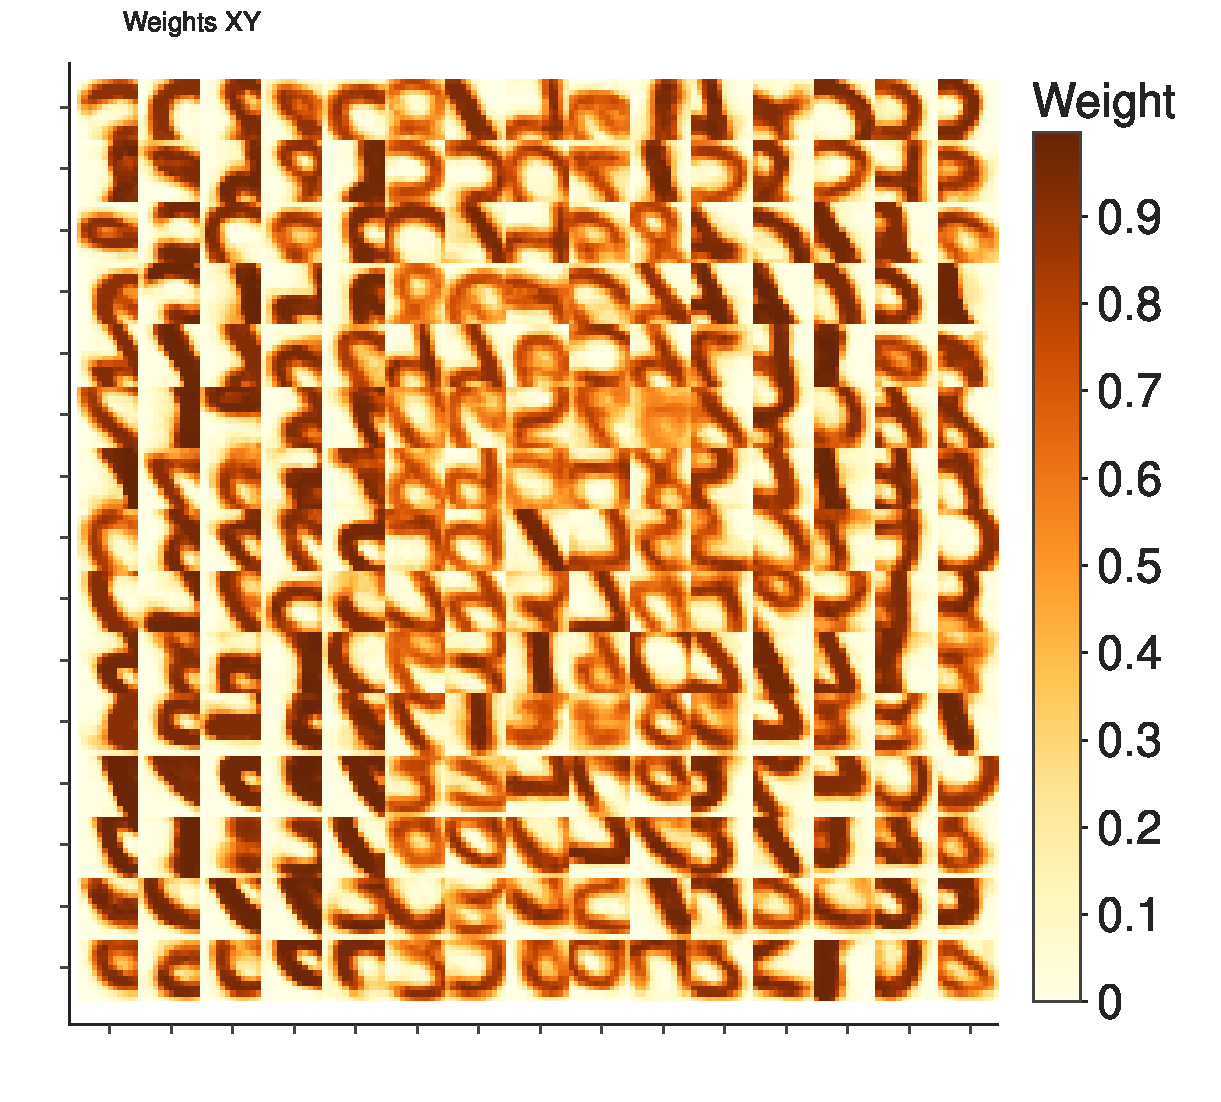
\includegraphics[width=\textwidth,keepaspectratio=true]{weights_XY_clamp_high.pdf}
    \caption{}
    \label{fig:compe_clamp:high_weights}
\end{subfigure}
\caption{Impact of limiting the values of inhibitory weights on accuracy. Figures \ref{fig:compe_clamp:low_weights} and \ref{fig:compe_clamp:high_weights} show $XY$ weights and Figures \ref{fig:compe_clamp:low_distr} and \ref{fig:compe_clamp:high_distr} show the competition ($YY$) weights distributions. The inhibitory weights were clamped (during training) to $[-350, 0]$ (Fig. \ref{fig:compe_clamp:low_distr},\subref{fig:compe_clamp:low_weights}) and to $(-\infty, -100]$ (Fig. \ref{fig:compe_clamp:high_distr},\subref{fig:compe_clamp:high_weights}). The accuracy of a network with the same hyperparameters, but without the competition limitation is 82.3\%, which is significantly higher than the accuracies of the networks presented in this Figure. Its weights $ XY $ are shown in Fig. \ref{fig:best_competition_XY}, and the distribution of its inhibitory weights is shown in Fig. \ref{fig:competition_distributions:strong}. In both cases the networks develop more blurred features comparing to the network with unrestricted competition in Fig. \ref{fig:competition_distributions:strong}
} 
\label{fig:compe_clamp}
\end{figure}

Competition training made it possible to achieve an accuracy slightly (by 2 \%) higher than the accuracy of a network of the same configuration, but with a fixed competition with inhibitory weights equal to $ -50 $ (Table \ref{results}, №4 and №5).

\section{Discussion}
This study demonstrates that a locally connected network is a promising spiked neural network architecture suitable for efficient implementation on a specialized neural hardware. Indeed, the ability to quickly plateau the learning curve allows the LCSNN to be used for training on relatively small training samples (3000-5000). The use of an additional activity interpretation algorithm, such as a linear classifier, can improve the efficiency of the network. Note that in this case the very features of the objects being recognized are learned by the network in an unsupervised fashion. The question remains about the possibility of obtaining similar results without using supervised learning to interpret network activity.

The main advantage of LCSNN is, as has been shown, that the locally connected network outperforms the convolutional in accuracy with approximately the same or slightly larger number of parameters. Presumably, this is due to the richer statistics of patches (receptive fields) that neurons within each channel respond to, compared to one receptive field per channel in the convolutional architecture. The price for this is the increased number of network parameters, but is not a critical factor due to the local (as opposed to fully connected) topology of interneural contacts. The local architecture also allows to save information about the localization of the selected feature in space and therefore is a reasonable choice for the implementation of unsupervised trained SNNs. This choice also determines its overall efficiency (in terms of performance, accuracy and power consumption at a certain density of elements) in a hardware implementation, in which each weight is usually represented by one or more physical elements (mainly SRAM cells \parencite{TrueNorth, Loihi} or memristors \parencite{Li_2018}).
The training of inhibitory connections slightly increases the accuracy of the LCSNN-based algorithm, but it is not so critical as to justify the use of such an expensive operation as the introduction and training of a significant number of inhibitory connections with finite weights of different values. At the same time, this conclusion is probably only valid only for small networks, like the one studied in this paper. In our opinion, the selection of optimal algorithms and parameters for training competition for deep SNNs deserves a more thorough study, in which the balance of competition and cooperation of neurons within each layer can lead to the formation of clusters from classes of supplied images, which contributes to building a semantically-like hierarchy of learned features and their combinations, that is, the final images \parencite{10.1007/978-3-030-30425-6_30}. Potentially, such a hierarchy of images can lead to a significant increase in the quality metrics.

\clearpage

\addcontentsline{toc}{section}{Conclusion}
\section*{Conclusion}
It was shown that for the problem of pattern recognition on the MNIST dataset, the locally connected architecture with competition is superior to the convolutional one with an equal number of parameters.
It was also shown that training inhibitory weights can slightly improve the quality of the model, and in the resulting distribution of inhibitory weights, both with high values (strong competition) and low (cooperation) values of weights are important.

\pagebreak

\printbibliography[sorting=nyt,heading=bibintoc,type=article,title={References}]
 
\end{document}  
